\documentclass[12pt,a4paper]{article}

% Package to include code
\usepackage{listings}
\usepackage{color}
\lstset{language=Python}
\lstset{numbers=none, basicstyle=\footnotesize,
  numberstyle=\tiny,keywordstyle=\color{blue},stringstyle=\ttfamily,showstringspaces=false}
\lstset{backgroundcolor=\color[rgb]{0.95 0.95 0.95}}
\lstdefinestyle{numbers}{numbers=left, stepnumber=1, numberstyle=\tiny, numbersep=10pt}
\lstdefinestyle{nonumbers}{numbers=none}


% Font selection: uncomment the next line to use the ``beton'' font
%\usepackage{beton}

% Font selection: uncomment the next line to use the ``times'' font
%\usepackage{times}

% Font for equations
\usepackage{euler}


%Package to define the headers and footers of the pages
\usepackage{fancyhdr}


%Package to include an index
\usepackage{index}

%Package to display boxes around texts. Used especially for the internal notes.
\usepackage{framed}

%PSTricks is a collection of PostScript-based TEX macros that is compatible
% with most TEX macro packages
\usepackage{pstricks}
\usepackage{pst-node}
\usepackage{pst-plot}
\usepackage{pst-tree}

%Package to display boxes around a minipage. Used especially to
%describe the biography of people.
\usepackage{boxedminipage}

%Package to include postscript figures
\usepackage{epsfig}

%Package for the bibliography
% \cite{XXX} produces Ben-Akiva et. al., 2010
% \citeasnoun{XXX} produces Ben-Akiva et al. (2010)
% \citeasnoun*{XXX} produces Ben-Akiva, Bierlaire, Bolduc and Walker (2010)
\usepackage[dcucite,abbr]{harvard}
\harvardparenthesis{none}\harvardyearparenthesis{round}

%Packages for advanced mathematics typesetting
\usepackage{amsmath,amsfonts,amssymb}

%Package to display trees easily
%\usepackage{xyling}

%Package to include smart references (on the next page, on the
%previous page, etc.) 
%%

%% Remove as it is not working when the book will be procesed by the
%% publisher.
%\usepackage{varioref}

%Package to display the euro sign
\usepackage[right,official]{eurosym}

%Rotate material, especially large table (defines sidewaystable)
\usepackage[figuresright]{rotating}

%Defines the subfigure environment, to obtain refs like Figure 1(a)
%and Figure 1(b). 
\usepackage{subfigure}

%Package for appendices. Allows subappendices, in particular
\usepackage{appendix}

%Package controling the fonts for the captions
\usepackage[font={small,sf}]{caption}

%Defines new types of columns for tabular ewnvironment
\usepackage{dcolumn}
\newcolumntype{d}{D{.}{.}{-1}}
\newcolumntype{P}[1]{>{#1\hspace{0pt}\arraybackslash}}
\newcolumntype{.}{D{.}{.}{9.3}}

%Allows multi-row cells in tables
\usepackage{multirow}

%Tables spaning more than one page
\usepackage{longtable}


%%
%%  Macros by Michel
%%

%Internal notes
\newcommand{\note}[1]{
\begin{framed}{}%
\textbf{\underline{Internal note}:} #1
\end{framed}}

%Use this version to turn off the notes
%\newcommand{\note}[1]{}


%Include a postscript figure . Note that the label is prefixed with
%``fig:''. Remember it when you refer to it.  
%Three arguments:
% #1 label
% #2 file (without extension)
% #3 Caption
\newcommand{\afigure}[3]{%
\begin{figure}[!tbp]%
\begin{center}%
\epsfig{figure=#2,width=0.8\textwidth}%
\end{center}
\caption{\label{fig:#1} #3}%
\end{figure}}






%Include two postscript figures side by side. 
% #1 label of the first figure
% #2 file for the first figure
% #3 Caption for the first figure
% #4 label of the second figure
% #5 file for the second figure
% #6 Caption for the first figure
% #7 Caption for the set of two figures
\newcommand{\twofigures}[7]{%
\begin{figure}[htb]%
\begin{center}%
\subfigure[\label{fig:#1}#3]{\epsfig{figure=#2,width=0.45\textwidth}}%
\hfill
\subfigure[\label{fig:#4}#6]{\epsfig{figure=#5,width=0.45\textwidth}}%
\end{center}
\caption{#7}%
\end{figure}}

%Include a figure generated by gnuplot using the epslatex output. Note that the label is prefixed with
%``fig:''. Remember it when you refer to it.  
 
%Three arguments:
% #1 label
% #2 file (without extension)
% #3 Caption
\newcommand{\agnuplotfigure}[3]{%
\begin{figure}[!tbp]%
\begin{center}%
\input{#2}%
\end{center}
\caption{\label{fig:#1} #3}%
\end{figure}}

%Three arguments:
% #1 label
% #2 file (without extension)
% #3 Caption
\newcommand{\asidewaysgnuplotfigure}[3]{%
\begin{sidewaysfigure}[!tbp]%
\begin{center}%
\input{#2}%
\end{center}
\caption{\label{fig:#1} #3}%
\end{sidewaysfigure}}


%Include two postscript figures side by side. 
% #1 label of the first figure
% #2 file for the first figure
% #3 Caption for the first figure
% #4 label of the second figure
% #5 file for the second figure
% #6 Caption for the second figure
% #7 Caption for the set of two figures
% #8 label for the whole figure
\newcommand{\twognuplotfigures}[7]{%
\begin{figure}[htb]%
\begin{center}%
\subfigure[\label{fig:#1}#3]{\input{#2}}%
\hfill
\subfigure[\label{fig:#4}#6]{\input{#5}}%
\end{center}
\caption{#7}%
\end{figure}}



%Include the description of somebody. Four arguments:
% #1 label
% #2 Name
% #3 file (without extension)
% #4 description
\newcommand{\people}[4]{
\begin{figure}[tbf]
\begin{boxedminipage}{\textwidth}
\parbox{0.40\textwidth}{\epsfig{figure=#3,width = 0.39\textwidth}}%\hfill
\parbox{0.59\textwidth}{%
#4% 
}%
\end{boxedminipage}
\caption{\label{fig:#1} #2}
\end{figure}
}

%Default command for a definition
% #1 label (prefix def:)
% #2 concept to be defined
% #3 definition
\newtheorem{definition}{Definition}
\newcommand{\mydef}[3]{%
\begin{definition}%
\index{#2|textbf}%
\label{def:#1}%
\textbf{#2} \slshape #3\end{definition}}

%Reference to a definitoin. Prefix 'def:' is assumed
\newcommand{\refdef}[1]{definition~\ref{def:#1}}


%Default command for a theorem, with proof
% #1: label (prefix thm:)
% #2: name of the theorem
% #3: statement
% #4: proof
\newtheorem{theorem}{Theorem}
\newcommand{\mytheorem}[4]{%
\begin{theorem}%
\index{#2|textbf}%
\index{Theorems!#2}%
\label{thm:#1}%
\textbf{#2} \sffamily \slshape #3
\end{theorem} \bpr #4 \epr \par}


%Default command for a theorem, without proof
% #1: label (prefix thm:)
% #2: name of the theorem
% #3: statement
\newcommand{\mytheoremsp}[3]{%
\begin{theorem}%
\index{#2|textbf}%
\index{Theorems!#2}%
\label{thm:#1}%
\textbf{#2} \sffamily \slshape #3
\end{theorem}}



%Put parentheses around the reference, as standard for equations
\newcommand{\req}[1]{(\ref{#1})}

%Short cut to make a column vector in math environment (centered)
\newcommand{\cvect}[1]{\left( \begin{array}{c} #1 \end{array} \right) }

%Short cut to make a column vector in math environment (right justified)
\newcommand{\rvect}[1]{\left( \begin{array}{r} #1 \end{array} \right) }

%A reference to a theorem. Prefix thm: is assumed for the label.
\newcommand{\refthm}[1]{theorem~\ref{thm:#1}}

%Reference to a figure. Prefix fig: is assumed for the label.
\newcommand{\reffig}[1]{Figure~\ref{fig:#1}}

%Smart reference to a figure. Prefix fig: is assumed for the label.
%\newcommand{\vreffig}[1]{Figure~\vref{fig:#1}}

%C in mathcal font for the choice set
\newcommand{\C}{\mathcal{C}}

%R in bold font for the set of real numbers
\newcommand{\R}{\mathbb{R}}

%N in bold font for the set of natural numbers
\newcommand{\N}{\mathbb{N}}

%C in mathcal font for the log likelihood
\renewcommand{\L}{\mathcal{L}}

%S in mathcal font for the subset S
\renewcommand{\S}{\mathcal{S}}

%To write an half in math envionment
\newcommand{\half}{\frac{1}{2}}

%Probability
\newcommand{\prob}{\operatorname{Pr}}

%Expectation
\newcommand{\expect}{\operatorname{E}}

%Variance
\newcommand{\var}{\operatorname{Var}}

%Covariance
\newcommand{\cov}{\operatorname{Cov}}

%Correlation
\newcommand{\corr}{\operatorname{Corr}}

%Span
\newcommand{\myspan}{\operatorname{span}}

%plim
\newcommand{\plim}{\operatorname{plim}}

%Displays n in bold (for the normal distribution?)
\newcommand{\n}{{\bf n}}

%Includes footnote in a table environment. Warning: the footmark is
%always 1.
\newcommand{\tablefootnote}[1]{\begin{flushright}
\rule{5cm}{1pt}\\
\footnotemark[1]{\footnotesize #1}
\end{flushright}
}

%Defines the ``th'' as in ``19th'' to be a superscript
\renewcommand{\th}{\textsuperscript{th}}

%Begin and end of a proof
\newcommand{\bpr}{{\bf Proof.} \hspace{1 em}}
\newcommand{\epr}{$\Box$}


\title{Estimating choice models with latent variables with PythonBiogeme}
\author{Michel Bierlaire} 
\date{June 28, 2016}

\newcommand{\PBIOGEME}{PythonBiogeme}


\begin{document}


\begin{titlepage}
\pagestyle{empty}

\maketitle
\vspace{2cm}

\begin{center}
\small Report TRANSP-OR 160628 \\ Transport and Mobility Laboratory \\ School of Architecture, Civil and Environmental Engineering \\ Ecole Polytechnique F\'ed\'erale de Lausanne \\ \verb+transp-or.epfl.ch+
\begin{center}
\textsc{Series on Biogeme}
\end{center}
\end{center}


\clearpage
\end{titlepage}

The package PythonBiogeme (\texttt{biogeme.epfl.ch}) is designed to
estimate the parameters of various models using maximum likelihood
estimation. It is particularly designed for discrete choice models. In
this document, we present how to estimate choice models involving
latent variables. We assume that the reader is already familiar with
discrete choice models, with latent variables, and with \PBIOGEME.
 This document has been written using
\PBIOGEME\ 2.5, but should remain valid for future versions.  

\section{Models and notations}

The literature on discrete choice models with latent variables is vast
(\cite{walker2001extended}, \cite{ashok2002extending},
\cite{greene2003latent}, \cite{ben2002integration}, to cite just a
few). We start this document by a short introduction to the models and
the notations. 

A latent variable is a variable that cannot be directly
observed. Therefore, it is a random variable,
 usually characterized by a \textbf{structural} equation:
\begin{equation}
\label{eq:structural}
x^* = h(x;\beta^s) + \varepsilon^s,
\end{equation}
where $x$ is a vector of  explanatory variables (observed or latent), $\beta^s$ is
a vector of $K_s$ parameters (to be estimated from data) and $\varepsilon^s$
is the (random) error term. Note that the most common specification
for the function $h$ is linear:
\begin{equation}
h(x;\beta^s) = \beta_0^s + \sum_{k=1}^{K_s-1} \beta^s_k x_k.
\end{equation}
 In discrete choice, the utility $U_{in}$ that an individual $n$
 associates with an alternative $i$ is a latent variable.

The analyst obtains information about latent variables from indirect
measurements. They are manifestations of the underlying latent
entity.  For example, in discrete choice, utility is not observed, but
is estimated from the observation of actual choices. The relationship
between a latent variable and measurements is characterized by 
\textbf{measurement} equations.


The first type of measurement equation is designed to capture
potential biases occurring  when the latent variable is
reported. 
The measurement equation has the following form:
\begin{equation}
\label{eq:continuousMeasurement}
z = m(x^*,y;\beta^m) + \varepsilon^m,
\end{equation}
where $z$ is the reported value, $x^*$ is the latent variable, $y$ is a vector of observed explanatory
variables, $\beta^m$ is
a vector of $K_m$ parameters (to be estimated from data) and $\varepsilon^m$
is the (random) error term. Note that the most common specification
for the function $m$ is linear:
\begin{equation}
m(x^*,y;\beta^m) = \beta^m_0 x^* + \sum_{k=1}^{K_m-1} \beta^m_k y_k.
\end{equation}
Another measurement equation is necessary when  discrete ordered
variables are available. It is typical in our context. First, the
choice, as indicator of the utility of an alternative, is a binary
variable (the alternative is chosen or not).  Second, psychometric
indicators revealing latent variables associated with attitudes and
perceptions are most of the time coded using a Likert scale (\cite{likert1932technique}).
Suppose that the measurement is represented by an ordered discrete variable $I$
taking the values $j_1$, $j_2$, \ldots , $j_M$,  we have 
\begin{equation}
\label{eq:discreteMeas-b}
I = \left\{
\begin{array}{ll}
j_1 & \text{if } z < \tau_1 \\
j_2 & \text{if } \tau_1 \leq z < \tau_2 \\
& \vdots \\
j_i & \text{if } \tau_{i-1} \leq z < \tau_i \\
& \vdots \\
j_M & \text{if } \tau_{M-1} \leq z
\end{array}
\right.
\end{equation}
where $z$ is defined by \req{eq:continuousMeasurement}, and $\tau_1$, \ldots. $\tau_{M-1}$ are parameters to be estimated,
such that
\begin{equation}
\label{eq:discreteMeas-c}
\tau_1 \leq \tau_2 \leq \cdots \leq \tau_i \leq \cdots \leq \tau_{M-1}. 
\end{equation}
The probability of a given response $j_i$ is
\begin{equation}
\label{eq:discreteMeas-d}
\prob(j_i) = \prob(\tau_{i-1} < z \leq \tau_i) =  \prob(\tau_{i-1} \leq z \leq \tau_i) =
F_{\varepsilon^m}(\tau_i) - F_{\varepsilon^m}(\tau_{i-1}),
\end{equation}
where $F_{\varepsilon^m}$ is the cumulative distribution function
(CDF) of the error term $\varepsilon^m$. When a normal
distribution is assumed, the model \req{eq:discreteMeas-d} is called \emph{ordered probit}. 

Note that the Likert scale, as proposed by \citeasnoun{likert1932technique}, has $M=5$ levels: 
\begin{enumerate}
\item strongly approve,
\item approve,
\item undecided,
\item disapprove,
\item strongly disapprove. 
\end{enumerate}

In the choice context, there are two categories: chosen, or not
chosen, so that $M=2$. Considering alternative $i$ for individual $n$,
the variable $z_{in}$ is the difference
\begin{equation}
z_{in} = U_{in} - \max_{j} U_{jn}
\end{equation}
 between the utility of alternative $i$ and the largest utility among all
alternatives, so that
\begin{equation}
I_{in}= \left\{
\begin{array}{ll}  
0 & \text{if } z_{in} < 0 \\
1 & \text{if } z_{in} \geq 0 \\
\end{array}
\right.
\end{equation}
which is \req{eq:discreteMeas-b} with $M=2$ and $\tau_1=0$.


\section{Indirect measurement of latent variables}

The indirect measurement of latent variables is usually done by
collecting various indicators. A list of statements is provided to the
respondent, and she is asked to react to each of them using a Likert scale, as
defined above. Although these statements have been designed to capture
some pre-determined aspects, it is useful to identify what are the
indicators that reveal most of the information about the latent
variables. 

We consider an example based on data collected in Switzerland in 2009
and 2010 (\cite{AtaGleBier_ICMC2011}, \cite{AtaGlerBier2012_DISP}). Various indicators, revealing various attitudes about the
environment, about mobility, about residential preferences, and about
lifestyle, have been collected, as described in Table~\ref{tab:indic}.

We first perform an exploratory factor analysis on the indicators. For
instance, the code in Section~\ref{sec:factoranalysis} performs this
task using the package R (\verb+www.r-project.org+). 

The results are
\begin{lstlisting}
          Factor1 Factor2 Factor3
Envir01   -0.565                 
Envir02   -0.407                 
Envir03    0.414                 
Mobil11    0.484                 
Mobil14    0.473                 
Mobil16    0.462                 
Mobil17    0.434                 
Mobil26                    0.408 
ResidCh01          0.577         
ResidCh04          0.406         
ResidCh05          0.635         
ResidCh06          0.451         
ResidCh07         -0.418         
LifSty07           0.430         
\end{lstlisting}

The first factor is explained by the following indicators: 
\begin{description}
\item[Envir01] Fuel price should be increased to reduce congestion and air pollution. 
\item[Envir02] More public transportation is needed, even if taxes are set to pay the additional costs.
\item[Envir03] Ecology disadvantages minorities and small businesses.
\item[Mobil11]  It is difficult to take the public transport when I carry bags or luggage.
\item[Mobil14]  When I take the car I know I will be on time.
\item[Mobil16] I do not like changing the mean of transport when I am
  traveling.
\item[Mobil17] If I use public transportation I have to cancel certain activities I would have done if I had taken the car.
\end{description}

We decide to label the associated latent variable ``car lover''. Note
the sign of the loading factors, and the associated interpretation of
the statements. 

In order to write the structural equation \req{eq:structural}, we
first define some variables from the data file. 

\begin{itemize}
\item \lstinline+age_65_more+: the respondent is 65 or older;
\item \lstinline+moreThanOneCar+: the number of cars in the household is
  strictly greater than 1;
\item \lstinline+moreThanOneBike+: the number of bikes in the household is
  strictly greater than 1;
\item \lstinline+individualHouse+: the type of house is individual or terraced;
\item \lstinline+male+: the respondent is a male;
\item \lstinline+haveChildren+: the family is a couple or a single with children;
\item \lstinline+haveGA+: the respondent owns a season ticket;
\item \lstinline+highEducation+: the respondent has obtained a degree
  strictly higher than high school.
\end{itemize}

We also want to include income. As it is a continuous variable, and
strict linearity is not appropriate, we adopt a piecewise linear (or
spline) specification. To do so, we define the following variables:

\begin{itemize}
\item \lstinline+ScaledIncome+: income, in 1000 CHF;
\item \lstinline+ContIncome_0_4000+:  min(\lstinline+ScaledIncome+,4)
\item \lstinline+ContIncome_4000_6000+: max(0,min(\lstinline+ScaledIncome+-4,2))
\item \lstinline+ContIncome_6000_8000+: max(0,min(\lstinline+ScaledIncome+-6,2))
\item \lstinline+ContIncome_8000_10000+: max(0,min(\lstinline+ScaledIncome+-8,2))
\item \lstinline+ContIncome_10000_more+: max(0,\lstinline+ScaledIncome+-10)
\end{itemize}

The structural equation is therefore
\begin{equation}
\label{eq:x_s}
\begin{array}{rcl}
x^* &=& \beta^s_0 + \sum_{k=1}^{13} \beta^s_k x_k + \sigma_s
\varepsilon^s \\
 &=& \bar{x}^s + \sigma_s \varepsilon^s,
\end{array}
\end{equation}
where $\varepsilon^s$ is a random variable normally distributed with
mean 0 and variance 1: 
\begin{equation}
\varepsilon^s \sim N(0,1),
\end{equation}
and
\begin{equation}
\bar{x}^s = \beta^s_0 + \sum_{k=1}^{13} \beta^s_k x_k.
\end{equation}
\subsection{Indicators as continuous variables}
\label{sec:continuous}
Consider now the measurement equations \req{eq:continuousMeasurement},
assuming that the indicators provided by the respondents are
continuous, that is that the indicators $I_i$ are used for $z$ in \req{eq:continuousMeasurement}. Although this is not formally correct, we assume it first
to present corresponding the formulation. We are describing the correct
way in Section~\ref{sec:discrete}. 

We define the measurement equation for indicator $i$ as 
\begin{equation}
\label{eq:x_m}
I_i =  \beta_{0i}^m +\beta^m_i x^* + \sigma^m_i \varepsilon^{m}_i,
\end{equation}
where 
\begin{equation}
\varepsilon^{m}_i \sim N(0,1).
\end{equation}
Using \req{eq:x_s} into \req{eq:x_m}, we obtain
\begin{equation}
\begin{array}{rcl}
I_i &=&  \beta_{0i}^m +\beta^m_i (\bar{x}^s + \sigma_s
\varepsilon^s)  + \sigma^m_i \varepsilon^{m}_i \\
  &=&  \beta_{0i}^m +\beta^m_i \bar{x}^s + \beta^m_i\sigma_s\varepsilon^s +  \sigma^m_i\varepsilon^{m}_i.
\end{array}
\end{equation}
The quantity
\begin{equation}
 \beta^m_i\sigma_s\varepsilon^s +  \sigma^m_i\varepsilon^{m}_i
\end{equation}
 is  normally distributed as
\begin{equation}
N\left(0,(\sigma_i^*)^2\right),
\end{equation}
where $(\sigma_i^*)^2 =(\beta^m_i\sigma_s)^2 +(\sigma^m_i)^2$. The parameter $\sigma_s$ is
normalized to 1, so that
\[
\begin{array}{rcl} 
(\sigma_i^*)^2 & =&(\beta^m_i\sigma_s)^2 +(\sigma^m_i)^2 \\
               & =&(\beta^m_i)^2 +(\sigma^m_i)^2,
\end{array}
\]
and
 \[
\sigma^m_i = \sqrt{(\sigma_i^*)^2 - (\beta^m_i)^2}.
\]
 Therefore, we rewrite the
measurement equations as 
\begin{equation}
\label{eq:measurementCoded}
I_i =  \beta_{0i}^m +\beta^m_i \bar{x}^s + \sigma^*_i \varepsilon_i^*,
\end{equation}
where $\varepsilon_i^* \sim N(0,1)$.
Not all these parameters can be estimated from data. We need to set
the units of the  latent variable. It is decided to set it to the
first indicator ($i=1$), by normalizing
  $\beta_{01}=0$ and $\beta^m_1 = -1$. 
Note the $-1$ coefficient, capturing the fact that the first indicator
increases when the car loving attitude \textbf{decreases}, as revealed
by the factor analysis results, and confirmed by the interpretation. 

The implementation of this model in \PBIOGEME\ is reported in
Section~\ref{sec:01oneLatentRegression}. 

The statement 
\begin{lstlisting}
loglikelihoodregression(Envir01,MODEL_Envir01,SIGMA_STAR_Envir01)
\end{lstlisting}
provides the log likelihood for the linear regression, where
\lstinline$Envir01$ is the dependent variable $I_i$,
\lstinline$MODEL_Envir01$ is the model $\beta_{0i}^m +\beta^m_i
\bar{x}^s$, \lstinline$CARLOVERS$ is $\bar{x}^s$ and
\lstinline$SIGMA_STAR_Envir01$ is the scale parameter $\sigma_i^*$. Note that there are
missing data. If the dependent variable is not positive or equal to 6, the value
should be ignored and the log
likelihood set to 0. This is implemented using the following
statement: 
\begin{lstlisting}
Elem({0:0, \
 1:loglikelihoodregression(Envir01,MODEL_Envir01,SIGMA_STAR_Envir01)},\
  (Envir01 > 0)*(Envir01 < 6)) 
\end{lstlisting}
The dictionary \lstinline$F$ gathers, for each respondent, the log
likelihood of the 7 indicators. The statement 
\begin{lstlisting}
loglike = bioMultSum(F)
\end{lstlisting}
calculates the total log likelihood for a given respondent of all 7
indicators together. 

The estimation results are reported in Tables~\ref{tab:regression} and
\ref{tab:regression2}, where for each indicator $i$,
\begin{itemize}
\item \lstinline$INTER_i$ is the intercept $\beta_{0i}^m$,
\item \lstinline$B_i$ is the coefficient $\beta^m_i$,
\item \lstinline$SIGMA_STAR_i$ is the scale $\sigma_i^*$,
\end{itemize}
in \req{eq:measurementCoded}.

\begin{table}[htb]
\caption{\label{tab:regression}Estimation results for the linear regression}
  \begin{tabular}{l}
\begin{tabular}{rlr@{.}lr@{.}lr@{.}lr@{.}l}
         &                       &   \multicolumn{2}{l}{}    & \multicolumn{2}{l}{Robust}  &     \multicolumn{4}{l}{}   \\
Parameter &                       &   \multicolumn{2}{l}{Coeff.}      & \multicolumn{2}{l}{Asympt.}  &     \multicolumn{4}{l}{}   \\
number &  Description                     &   \multicolumn{2}{l}{estimate}      & \multicolumn{2}{l}{std. error}  &   \multicolumn{2}{l}{$t$-stat}  &   \multicolumn{2}{l}{$p$-value}   \\

\hline

1 & \lstinline$INTER_Envir02$ & 2&01 & 0&153 & 13&10 & 0&00\\
2 & \lstinline$INTER_Envir03$ & 4&57 & 0&158 & 28&85 & 0&00\\
3 & \lstinline$INTER_Mobil11$ & 5&14 & 0&151 & 34&04 & 0&00\\
4 & \lstinline$INTER_Mobil14$ & 4&91 & 0&157 & 31&21 & 0&00\\
5 & \lstinline$INTER_Mobil16$ & 4&80 & 0&158 & 30&28 & 0&00\\
6 & \lstinline$INTER_Mobil17$ & 4&50 & 0&157 & 28&64 & 0&00\\
7 & \lstinline$L_Envir02_F1$ & -0&496 & 0&0578 & -8&59 & 0&00\\
8 & \lstinline$L_Envir03_F1$ & 0&671 & 0&0601 & 11&16 & 0&00\\
9 & \lstinline$L_Mobil11_F1$ & 0&563 & 0&0589 & 9&56 & 0&00\\
10 & \lstinline$L_Mobil14_F1$ & 0&705 & 0&0596 & 11&83 & 0&00\\
11 & \lstinline$L_Mobil16_F1$ & 0&540 & 0&0612 & 8&82 & 0&00\\
12 & \lstinline$L_Mobil17_F1$ & 0&432 & 0&0600 & 7&20 & 0&00\\
13 & \lstinline$SIGMA_STAR_Envir01$ & 1&25 & 0&0161 & 77&34 & 0&00\\
14 & \lstinline$SIGMA_STAR_Envir02$ & 1&12 & 0&0149 & 75&04 & 0&00\\
15 & \lstinline$SIGMA_STAR_Envir03$ & 1&07 & 0&0155 & 68&92 & 0&00\\
16 & \lstinline$SIGMA_STAR_Mobil11$ & 1&08 & 0&0163 & 66&40 & 0&00\\
17 & \lstinline$SIGMA_STAR_Mobil14$ & 1&05 & 0&0141 & 74&62 & 0&00\\
18 & \lstinline$SIGMA_STAR_Mobil16$ & 1&10 & 0&0151 & 72&55 & 0&00\\
19 & \lstinline$SIGMA_STAR_Mobil17$ & 1&11 & 0&0155 & 71&74 & 0&00\\
\end{tabular}
  \end{tabular}
\end{table}

\begin{table}[htb]
\caption{\label{tab:regression2}Estimation results for the linear
  regression (ctd)}
  \begin{tabular}{l}
\begin{tabular}{rlr@{.}lr@{.}lr@{.}lr@{.}l}
         &                       &   \multicolumn{2}{l}{}    & \multicolumn{2}{l}{Robust}  &     \multicolumn{4}{l}{}   \\
Parameter &                       &   \multicolumn{2}{l}{Coeff.}      & \multicolumn{2}{l}{Asympt.}  &     \multicolumn{4}{l}{}   \\
number &  Description                     &   \multicolumn{2}{l}{estimate}      & \multicolumn{2}{l}{std. error}  &   \multicolumn{2}{l}{$t$-stat}  &   \multicolumn{2}{l}{$p$-value}   \\

\hline

20 & \lstinline$coef_ContIncome_0_4000$ & 0&103 & 0&0633 & 1&63 & 0&10\\
21 & \lstinline$coef_ContIncome_10000_more$ & 0&103 & 0&0360 & 2&86 & 0&00\\
22 & \lstinline$coef_ContIncome_4000_6000$ & -0&252 & 0&108 & -2&33 & 0&02\\
23 & \lstinline$coef_ContIncome_6000_8000$ & 0&300 & 0&130 & 2&31 & 0&02\\
24 & \lstinline$coef_ContIncome_8000_10000$ & -0&621 & 0&150 & -4&13 & 0&00\\
25 & \lstinline$coef_age_65_more$ & 0&103 & 0&0732 & 1&41 & 0&16\\
26 & \lstinline$coef_haveChildren$ & -0&0454 & 0&0542 & -0&84 & 0&40\\
27 & \lstinline$coef_haveGA$ & -0&689 & 0&0861 & -8&00 & 0&00\\
28 & \lstinline$coef_highEducation$ & -0&298 & 0&0612 & -4&87 & 0&00\\
29 & \lstinline$coef_individualHouse$ & -0&110 & 0&0540 & -2&04 & 0&04\\
30 & \lstinline$coef_intercept$ & -2&50 & 0&183 & -13&66 & 0&00\\
31 & \lstinline$coef_male$ & 0&0716 & 0&0506 & 1&41 & 0&16\\
32 & \lstinline$coef_moreThanOneBike$ & -0&328 & 0&0621 & -5&28 & 0&00\\
33 & \lstinline$coef_moreThanOneCar$ & 0&624 & 0&0581 & 10&74 & 0&00\\
\hline
\end{tabular}
\\
\begin{tabular}{rcl}
\multicolumn{3}{l}{\bf Summary statistics}\\
\multicolumn{3}{l}{ Number of observations = $1906$} \\
\multicolumn{3}{l}{ Number of excluded observations = $359$} \\
\multicolumn{3}{l}{ Number of estimated  parameters = $33$} \\
 $\mathcal{L}(\hat{\beta})$ &=& $-20658.648 $  \\
\end{tabular}
  \end{tabular}
\end{table}

\subsection{Indicators as discrete variables}
\label{sec:discrete}

We now consider the measurement equations
\req{eq:discreteMeas-b}.
As the measurements are using a Likert scale with $M=5$ levels, we
define 4 parameters $\tau_i$. In order to account for the symmetry of
the indicators, we actually define two positive parameters $\delta_1$ and
$\delta_2$, and define
\[
\begin{array}{rcl}
\tau_1 &=& -\delta_1 - \delta_2 \\
\tau_2 &=& -\delta_1 \\
\tau_3 &=& \delta_1 \\
\tau_4 &=& \delta_1 + \delta_2 \\
\end{array}
\]
Therefore, the probability of a given response is given by the ordered
probit model:
\begin{equation}
\label{eq:likelihoodOrderedProbit}
\begin{array}{rcl}
\prob(I_i = j_i) &=& \prob(\tau_{i-1} \leq z \leq \tau_i) \\ & \\
           &=& \prob(\tau_{i-1} \leq  \beta_{0i}^m +\beta^m_i \bar{x}^s +
\sigma^*_i \varepsilon_i^*  \leq \tau_i) \\ & \\
           &=& \prob\left(\frac{\tau_{i-1} - \beta_{0i}^m - \beta^m_i \bar{x}^s}{\sigma^*_i}
< 
 \varepsilon_i^*  \leq \frac{\tau_i - \beta_{0i}^m - \beta^m_i
 \bar{x}^s}{\sigma^*_i}\right) \\ & \\
&=&\Phi\left(\frac{\tau_i - \beta_{0i}^m - \beta^m_i
 \bar{x}^s}{\sigma^*_i}\right) - \Phi\left(\frac{\tau_{i-1} - \beta_{0i}^m - \beta^m_i \bar{x}^s}{\sigma^*_i}\right),
\end{array}
\end{equation}
where $\Phi(\cdot)$ is the CDF of the standardized normal
distribution, as illustrated in Figure~\ref{fig:ordinal}.

\begin{figure}[htb]
% GNUPLOT: LaTeX picture with Postscript
\begingroup
  \makeatletter
  \providecommand\color[2][]{%
    \GenericError{(gnuplot) \space\space\space\@spaces}{%
      Package color not loaded in conjunction with
      terminal option `colourtext'%
    }{See the gnuplot documentation for explanation.%
    }{Either use 'blacktext' in gnuplot or load the package
      color.sty in LaTeX.}%
    \renewcommand\color[2][]{}%
  }%
  \providecommand\includegraphics[2][]{%
    \GenericError{(gnuplot) \space\space\space\@spaces}{%
      Package graphicx or graphics not loaded%
    }{See the gnuplot documentation for explanation.%
    }{The gnuplot epslatex terminal needs graphicx.sty or graphics.sty.}%
    \renewcommand\includegraphics[2][]{}%
  }%
  \providecommand\rotatebox[2]{#2}%
  \@ifundefined{ifGPcolor}{%
    \newif\ifGPcolor
    \GPcolorfalse
  }{}%
  \@ifundefined{ifGPblacktext}{%
    \newif\ifGPblacktext
    \GPblacktexttrue
  }{}%
  % define a \g@addto@macro without @ in the name:
  \let\gplgaddtomacro\g@addto@macro
  % define empty templates for all commands taking text:
  \gdef\gplbacktext{}%
  \gdef\gplfronttext{}%
  \makeatother
  \ifGPblacktext
    % no textcolor at all
    \def\colorrgb#1{}%
    \def\colorgray#1{}%
  \else
    % gray or color?
    \ifGPcolor
      \def\colorrgb#1{\color[rgb]{#1}}%
      \def\colorgray#1{\color[gray]{#1}}%
      \expandafter\def\csname LTw\endcsname{\color{white}}%
      \expandafter\def\csname LTb\endcsname{\color{black}}%
      \expandafter\def\csname LTa\endcsname{\color{black}}%
      \expandafter\def\csname LT0\endcsname{\color[rgb]{1,0,0}}%
      \expandafter\def\csname LT1\endcsname{\color[rgb]{0,1,0}}%
      \expandafter\def\csname LT2\endcsname{\color[rgb]{0,0,1}}%
      \expandafter\def\csname LT3\endcsname{\color[rgb]{1,0,1}}%
      \expandafter\def\csname LT4\endcsname{\color[rgb]{0,1,1}}%
      \expandafter\def\csname LT5\endcsname{\color[rgb]{1,1,0}}%
      \expandafter\def\csname LT6\endcsname{\color[rgb]{0,0,0}}%
      \expandafter\def\csname LT7\endcsname{\color[rgb]{1,0.3,0}}%
      \expandafter\def\csname LT8\endcsname{\color[rgb]{0.5,0.5,0.5}}%
    \else
      % gray
      \def\colorrgb#1{\color{black}}%
      \def\colorgray#1{\color[gray]{#1}}%
      \expandafter\def\csname LTw\endcsname{\color{white}}%
      \expandafter\def\csname LTb\endcsname{\color{black}}%
      \expandafter\def\csname LTa\endcsname{\color{black}}%
      \expandafter\def\csname LT0\endcsname{\color{black}}%
      \expandafter\def\csname LT1\endcsname{\color{black}}%
      \expandafter\def\csname LT2\endcsname{\color{black}}%
      \expandafter\def\csname LT3\endcsname{\color{black}}%
      \expandafter\def\csname LT4\endcsname{\color{black}}%
      \expandafter\def\csname LT5\endcsname{\color{black}}%
      \expandafter\def\csname LT6\endcsname{\color{black}}%
      \expandafter\def\csname LT7\endcsname{\color{black}}%
      \expandafter\def\csname LT8\endcsname{\color{black}}%
    \fi
  \fi
    \setlength{\unitlength}{0.0500bp}%
    \ifx\gptboxheight\undefined%
      \newlength{\gptboxheight}%
      \newlength{\gptboxwidth}%
      \newsavebox{\gptboxtext}%
    \fi%
    \setlength{\fboxrule}{0.5pt}%
    \setlength{\fboxsep}{1pt}%
\begin{picture}(7200.00,5040.00)%
    \gplgaddtomacro\gplbacktext{%
      \csname LTb\endcsname%
      \put(5185,2889){\makebox(0,0)[l]{\strut{}$\operatorname{Pr}(I=4)=\operatorname{Pr}(\tau_{3} \leq z \leq  \tau_4)$}}%
      \put(1625,290){\makebox(0,0){\strut{}$\tau_1$}}%
      \put(3081,290){\makebox(0,0){\strut{}$\tau_2$}}%
      \put(4052,290){\makebox(0,0){\strut{}$\tau_3$}}%
      \put(5508,290){\makebox(0,0){\strut{}$\tau_4$}}%
    }%
    \gplgaddtomacro\gplfronttext{%
      \csname LTb\endcsname%
      \put(6206,154){\makebox(0,0){\strut{}$z^*$}}%
    }%
    \gplbacktext
    \put(0,0){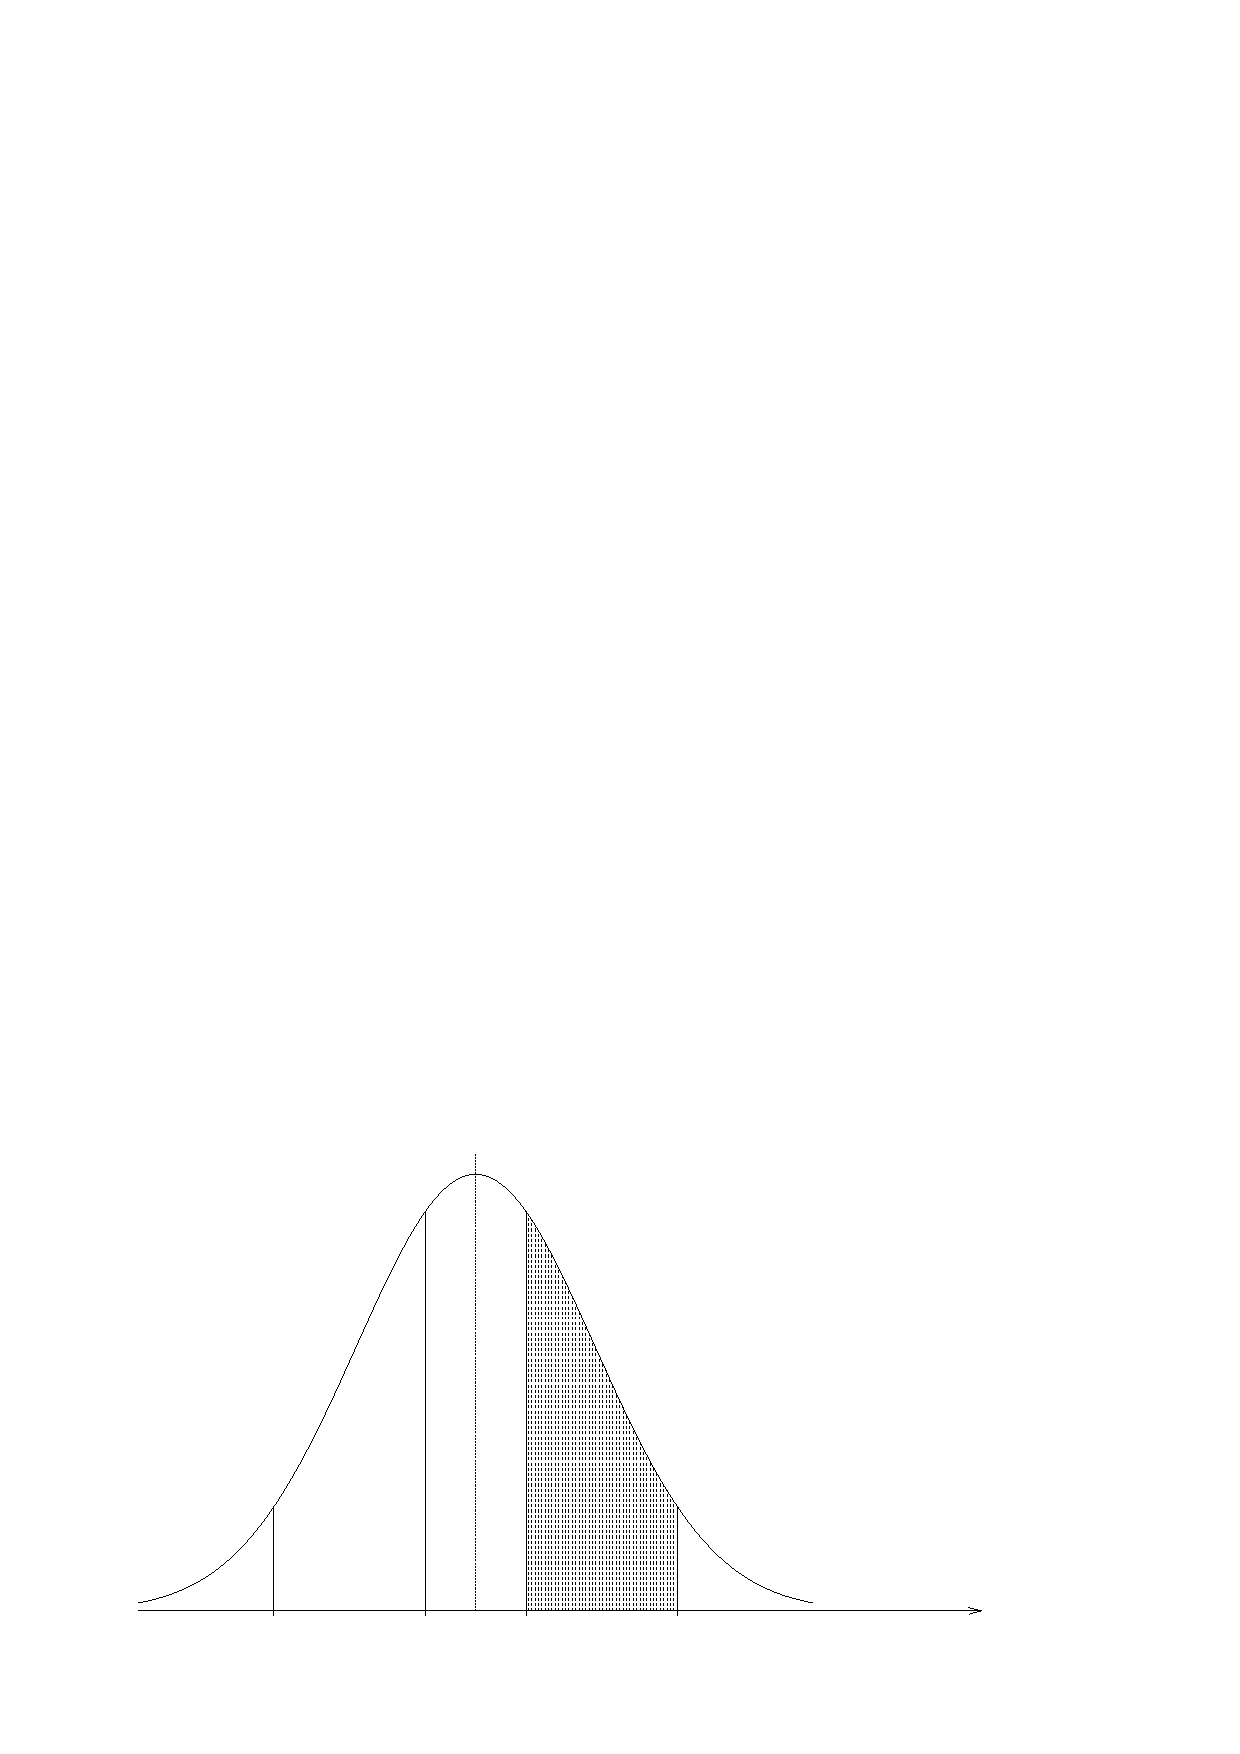
\includegraphics{fig-ordinal-1}}%
    \gplfronttext
  \end{picture}%
\endgroup

\caption{\label{fig:ordinal}Measurement equation for discrete indicators}
\end{figure}

The model specification for \PBIOGEME\ is reported in Section
\ref{sec:02oneLatentOrdered}. Equation~\ref{eq:likelihoodOrderedProbit}
is coded using the following statements:
\begin{lstlisting}
Envir01_tau_1 = (tau_1-MODEL_Envir01) / SIGMA_STAR_Envir01
Envir01_tau_2 = (tau_2-MODEL_Envir01) / SIGMA_STAR_Envir01
Envir01_tau_3 = (tau_3-MODEL_Envir01) / SIGMA_STAR_Envir01
Envir01_tau_4 = (tau_4-MODEL_Envir01) / SIGMA_STAR_Envir01
IndEnvir01 = {
    1: bioNormalCdf(Envir01_tau_1),
    2: bioNormalCdf(Envir01_tau_2)-bioNormalCdf(Envir01_tau_1),
    3: bioNormalCdf(Envir01_tau_3)-bioNormalCdf(Envir01_tau_2),
    4: bioNormalCdf(Envir01_tau_4)-bioNormalCdf(Envir01_tau_3),
    5: 1-bioNormalCdf(Envir01_tau_4),
    6: 1.0,
    -1: 1.0,
    -2: 1.0
}

P_Envir01 = Elem(IndEnvir01, Envir01)
\end{lstlisting}
Note that the indicators in the data file can take the values -2, -1, 1, 2,
3, 4, 5, and 6. However, the values 6, -1 and 2 are ignored, and
associated with a probability of 1, so that they have no influence on
the total likelihood function.

\begin{table}[htb]
\caption{\label{tab:ordered}Estimation results for the ordered probit
  regression}
  \begin{tabular}{l}
\begin{tabular}{rlr@{.}lr@{.}lr@{.}lr@{.}l}
         &                       &   \multicolumn{2}{l}{}    & \multicolumn{2}{l}{Robust}  &     \multicolumn{4}{l}{}   \\
Parameter &                       &   \multicolumn{2}{l}{Coeff.}      & \multicolumn{2}{l}{Asympt.}  &     \multicolumn{4}{l}{}   \\
number &  Description                     &   \multicolumn{2}{l}{estimate}      & \multicolumn{2}{l}{std. error}  &   \multicolumn{2}{l}{$t$-stat}  &   \multicolumn{2}{l}{$p$-value}   \\

\hline

1 & \lstinline$B_Envir02_F1$ & -0&431 & 0&0523 & -8&25 & 0&00\\
2 & \lstinline$B_Envir03_F1$ & 0&566 & 0&0531 & 10&66 & 0&00\\
3 & \lstinline$B_Mobil11_F1$ & 0&484 & 0&0533 & 9&09 & 0&00\\
4 & \lstinline$B_Mobil14_F1$ & 0&582 & 0&0514 & 11&34 & 0&00\\
5 & \lstinline$B_Mobil16_F1$ & 0&463 & 0&0543 & 8&53 & 0&00\\
6 & \lstinline$B_Mobil17_F1$ & 0&368 & 0&0519 & 7&10 & 0&00\\
7 & \lstinline$INTER_Envir02$ & 0&349 & 0&0261 & 13&35 & 0&00\\
8 & \lstinline$INTER_Envir03$ & -0&309 & 0&0270 & -11&42 & 0&00\\
9 & \lstinline$INTER_Mobil11$ & 0&338 & 0&0290 & 11&66 & 0&00\\
10 & \lstinline$INTER_Mobil14$ & -0&131 & 0&0251 & -5&21 & 0&00\\
11 & \lstinline$INTER_Mobil16$ & 0&128 & 0&0276 & 4&65 & 0&00\\
12 & \lstinline$INTER_Mobil17$ & 0&146 & 0&0260 & 5&60 & 0&00\\
13 & \lstinline$SIGMA_STAR_Envir02$ & 0&767 & 0&0222 & 34&62 & 0&00\\
14 & \lstinline$SIGMA_STAR_Envir03$ & 0&718 & 0&0206 & 34&89 & 0&00\\
15 & \lstinline$SIGMA_STAR_Mobil11$ & 0&783 & 0&0240 & 32&63 & 0&00\\
16 & \lstinline$SIGMA_STAR_Mobil14$ & 0&688 & 0&0209 & 32&98 & 0&00\\
17 & \lstinline$SIGMA_STAR_Mobil16$ & 0&754 & 0&0226 & 33&42 & 0&00\\
18 & \lstinline$SIGMA_STAR_Mobil17$ & 0&760 & 0&0235 & 32&32 & 0&00\\
\end{tabular}
  \end{tabular}
\end{table}

\begin{table}[htb]
\caption{\label{tab:ordered2}Estimation results for the ordered probit
  regression (ctd)}
  \begin{tabular}{l}
\begin{tabular}{rlr@{.}lr@{.}lr@{.}lr@{.}l}
         &                       &   \multicolumn{2}{l}{}    & \multicolumn{2}{l}{Robust}  &     \multicolumn{4}{l}{}   \\
Parameter &                       &   \multicolumn{2}{l}{Coeff.}      & \multicolumn{2}{l}{Asympt.}  &     \multicolumn{4}{l}{}   \\
number &  Description                     &   \multicolumn{2}{l}{estimate}      & \multicolumn{2}{l}{std. error}  &   \multicolumn{2}{l}{$t$-stat}  &   \multicolumn{2}{l}{$p$-value}   \\

\hline
19 & \lstinline$coef_ContIncome_0_4000$ & 0&0903 & 0&0528 & 1&71 & 0&09\\
20 & \lstinline$coef_ContIncome_10000_more$ & 0&0844 & 0&0303 & 2&79 & 0&01\\
21 & \lstinline$coef_ContIncome_4000_6000$ & -0&221 & 0&0918 & -2&41 & 0&02\\
22 & \lstinline$coef_ContIncome_6000_8000$ & 0&259 & 0&109 & 2&37 & 0&02\\
23 & \lstinline$coef_ContIncome_8000_10000$ & -0&523 & 0&128 & -4&10 & 0&00\\
24 & \lstinline$coef_age_65_more$ & 0&0717 & 0&0613 & 1&17 & 0&24\\
25 & \lstinline$coef_haveChildren$ & -0&0376 & 0&0459 & -0&82 & 0&41\\
26 & \lstinline$coef_haveGA$ & -0&578 & 0&0750 & -7&70 & 0&00\\
27 & \lstinline$coef_highEducation$ & -0&247 & 0&0521 & -4&73 & 0&00\\
28 & \lstinline$coef_individualHouse$ & -0&0886 & 0&0455 & -1&94 & 0&05\\
29 & \lstinline$coef_intercept$ & 0&398 & 0&153 & 2&61 & 0&01\\
30 & \lstinline$coef_male$ & 0&0664 & 0&0433 & 1&53 & 0&13\\
31 & \lstinline$coef_moreThanOneBike$ & -0&277 & 0&0538 & -5&15 & 0&00\\
32 & \lstinline$coef_moreThanOneCar$ & 0&533 & 0&0516 & 10&34 & 0&00\\
33 & \lstinline$delta_1$ & 0&252 & 0&00726 & 34&70 & 0&00\\
34 & \lstinline$delta_2$ & 0&759 & 0&0193 & 39&30 & 0&00\\
\hline
\end{tabular}
\\
\begin{tabular}{rcl}
\multicolumn{3}{l}{\bf Summary statistics}\\
\multicolumn{3}{l}{ Number of observations = $1906$} \\
\multicolumn{3}{l}{ Number of excluded observations = $359$} \\
\multicolumn{3}{l}{ Number of estimated  parameters = $34$} \\
 $\mathcal{L}(\hat{\beta})$ &=& $-17794.883 $  \\

\end{tabular}
  \end{tabular}

\end{table}


\clearpage

\section{Choice model}

Latent variables can be included in choice models. Consider a model
with three alternatives ``public transportation'' (PT), ``car'' (CAR)
and ``slow modes'' (SM). The utility functions are of the following form:
\begin{equation}
\label{eq:utility}
\begin{array}{rclclclcl}
U_{\text{PT}} &=& V_{\text{PT}} &+& \varepsilon_{\text{PT}} &=& \beta^t_\text{PT} \text{Time}_\text{PT} &+& \cdots + \varepsilon_{\text{PT}}\\
U_{\text{CAR}} &=&V_{\text{CAR}}&+& \varepsilon_{\text{CAR}} &=& \beta^t_\text{CAR} \text{Time}_\text{CAR} &+& \cdots
+ \varepsilon_{\text{CAR}}\\
U_{\text{SM}} &=&V_{\text{SM}} &+& \varepsilon_{\text{SM}}\\
\end{array}
\end{equation}
The full specification can be found in the specification
file in Section~\ref{sec:03choiceOnly}. 
 The
latent variable that we have considered in the previous sections captures the ``car loving'' attitude of the
individuals. In order to include it in the choice model, we specify that the coefficients
of travel time for the public transportation alternative, and for the
car alternative, vary with the latent variable. We have
\begin{equation}
\label{eq:beta_pt}
\beta^t_\text{PT} = \widehat{\beta}^t_\text{PT}
\exp(\beta^\text{CL}_\text{PT} x^*),
\end{equation}
and
\begin{equation}
\label{eq:beta_car}
\beta^t_\text{CAR} = \widehat{\beta}^t_\text{CAR}
\exp(\beta^\text{CL}_\text{CAR} x^*),
\end{equation}
where $x^*$ is defined by \req{eq:x_s}, so that
\begin{equation}
\beta^t_\text{PT} = \widehat{\beta}^t_\text{PT}
\exp(\beta^\text{CL}_\text{PT} (\bar{x}^s + \sigma_s \varepsilon^s)),
\end{equation}
and
\begin{equation}
\beta^t_\text{CAR} = \widehat{\beta}^t_\text{CAR}
\exp(\beta^\text{CL}_\text{CAR}(\bar{x}^s + \sigma_s \varepsilon^s)).
\end{equation}

Technically, such a choice model can be estimated using the choice observations
only, without the indicators. Assuming that $\varepsilon_{\text{PT}}$,
$\varepsilon_{\text{CAR}}$ and $\varepsilon_{\text{SM}}$ are
i.i.d. extreme value distributed, we have
\begin{equation}
\prob(\text{PT}|\varepsilon^s) = \frac{\exp(V_\text{PT})}{\exp(V_\text{PT})+\exp(V_\text{CAR})+\exp(V_\text{SM})} 
\end{equation}
and
\begin{equation}
\prob(\text{PT}) =
\int_{\varepsilon=-\infty}^{\infty}\prob(\text{PT}|\varepsilon)\phi(\varepsilon) d\varepsilon,
\end{equation}
where $\phi(\cdot)$ is the probability density function of
the univariate standardized normal
distribution.
The choice model is a mixture of logit models. The estimation results
are reported in Table~\ref{tab:choiceOnly}, where 
\begin{itemize}
\item \lstinline$BETA_TIME_PT_CL$ refers to $\beta^\protect\text{CL}_\protect\text{PT}$ in \req{eq:beta_pt},
\item \lstinline$BETA_TIME_PT_REF$ refers to $\widehat{\beta}^t_\protect\text{PT}$ in \req{eq:beta_pt},
\item \lstinline$BETA_TIME_CAR_CL$ refers to
  $\beta^\protect\text{CL}_\protect\text{CAR}$ in \req{eq:beta_car}, and
\item \lstinline$BETA_TIME_CAR_REF$ refers to $\widehat{\beta}^t_\protect\text{CAR}$ in \req{eq:beta_car}.
\end{itemize}

\begin{table}[htb]
\caption{\protect\label{tab:choiceOnly}Estimation results for the mixture of logit
models}
  \begin{tabular}{l}
\begin{tabular}{rlr@{.}lr@{.}lr@{.}lr@{.}l}
         &                       &   \multicolumn{2}{l}{}    & \multicolumn{2}{l}{Robust}  &     \multicolumn{4}{l}{}   \\
Parameter &                       &   \multicolumn{2}{l}{Coeff.}      & \multicolumn{2}{l}{Asympt.}  &     \multicolumn{4}{l}{}   \\
number &  Description                     &   \multicolumn{2}{l}{estimate}      & \multicolumn{2}{l}{std. error}  &   \multicolumn{2}{l}{$t$-stat}  &   \multicolumn{2}{l}{$p$-value}   \\

\hline

1 & \lstinline$ASC_CAR$ & 0&373 & 0&138 & 2&70 & 0&01\\
2 & \lstinline$ASC_SM$ & 0&964 & 0&263 & 3&66 & 0&00\\
3 & \lstinline$BETA_COST_HWH$ & -1&77 & 0&473 & -3&75 & 0&00\\
4 & \lstinline$BETA_COST_OTHER$ & -1&51 & 0&309 & -4&89 & 0&00\\
5 & \lstinline$BETA_DIST$ & -4&88 & 0&655 & -7&46 & 0&00\\
6 & \lstinline$BETA_TIME_CAR_CL$ & -0&491 & 0&0509 & -9&65 & 0&00\\
7 & \lstinline$BETA_TIME_CAR_REF$ & -27&1 & 6&17 & -4&39 & 0&00\\
8 & \lstinline$BETA_TIME_PT_CL$ & -1&75 & 0&0906 & -19&32 & 0&00\\
9 & \lstinline$BETA_TIME_PT_REF$ & -5&35 & 2&85 & -1&88 & 0&06\\
10 & \lstinline$BETA_WAITING_TIME$ & -0&0517 & 0&0175 & -2&96 & 0&00\\
11 & \lstinline$coef_ContIncome_0_4000$ & -0&102 & 0&0907 & -1&12 & 0&26\\
12 & \lstinline$coef_ContIncome_10000_more$ & -0&101 & 0&0354 & -2&86 & 0&00\\
13 & \lstinline$coef_ContIncome_4000_6000$ & 0&0272 & 0&121 & 0&22 & 0&82\\
14 & \lstinline$coef_ContIncome_6000_8000$ & -0&125 & 0&214 & -0&59 & 0&56\\
15 & \lstinline$coef_ContIncome_8000_10000$ & 0&326 & 0&188 & 1&73 & 0&08\\
16 & \lstinline$coef_age_65_more$ & 0&199 & 0&0858 & 2&32 & 0&02\\
17 & \lstinline$coef_haveChildren$ & -0&0414 & 0&0673 & -0&61 & 0&54\\
18 & \lstinline$coef_haveGA$ & 1&33 & 0&0869 & 15&30 & 0&00\\
19 & \lstinline$coef_highEducation$ & -0&462 & 0&0540 & -8&56 & 0&00\\
20 & \lstinline$coef_individualHouse$ & 0&115 & 0&124 & 0&92 & 0&36\\
21 & \lstinline$coef_male$ & -0&133 & 0&0567 & -2&35 & 0&02\\
22 & \lstinline$coef_moreThanOneBike$ & 0&152 & 0&0977 & 1&55 & 0&12\\
23 & \lstinline$coef_moreThanOneCar$ & -0&598 & 0&0669 & -8&94 & 0&00\\
\hline
\end{tabular}
\\
\begin{tabular}{rcl}
\multicolumn{3}{l}{\bf Summary statistics}\\
\multicolumn{3}{l}{ Number of observations = $1906$} \\
\multicolumn{3}{l}{ Number of excluded observations = $359$} \\
\multicolumn{3}{l}{ Number of estimated  parameters = $23$} \\
 $\mathcal{L}(\beta_0)$ &=&  $-2093.955$ \\
 $\mathcal{L}(\hat{\beta})$ &=& $-1078.003 $  \\
 $-2[\mathcal{L}(\beta_0) -\mathcal{L}(\hat{\beta})]$ &=& $2031.905$ \\
    $\rho^2$ &=&   $0.485$ \\
    $\bar{\rho}^2$ &=&    $0.474$ \\
\end{tabular}
  \end{tabular}
\end{table}


\clearpage 

\section{Sequential estimation}

In order to exploit both the choice data and the psychometric
indicator, we now combine the latent variable model with the choice
model. The easiest way to estimate a joint model is using sequential
estimation. However, such an estimator is not efficient, and a full
information estimation is preferable. It is described in Section~\ref{sec:fi}.

For the sequential estimation, we use \req{eq:x_s} in \req{eq:beta_pt} and
\req{eq:beta_car}, where the values of the coefficients $\beta^s$ are
the result of the estimation  presented in
Table~\ref{tab:ordered}. We have again a mixture of logit models, but
with fewer parameters, as the parameters of the structural equation
are not re-estimated. The specification file is presented in
Section~\ref{sec:04latentChoiceSeq}. The estimated parameters of the
choice model are presented in Table~\ref{tab:sequential}.

It is important to realize that the estimation results in
Tables~\ref{tab:choiceOnly} and \ref{tab:sequential} cannot be
compared, as they are not using the same data. 

 \begin{table}[htb]
\caption{\label{tab:sequential}Estimation results for the sequential estimation}
  \begin{tabular}{l}
\begin{tabular}{rlr@{.}lr@{.}lr@{.}lr@{.}l}
         &                       &   \multicolumn{2}{l}{}    & \multicolumn{2}{l}{Robust}  &     \multicolumn{4}{l}{}   \\
Parameter &                       &   \multicolumn{2}{l}{Coeff.}      & \multicolumn{2}{l}{Asympt.}  &     \multicolumn{4}{l}{}   \\
number &  Description                     &   \multicolumn{2}{l}{estimate}      & \multicolumn{2}{l}{std. error}  &   \multicolumn{2}{l}{$t$-stat}  &   \multicolumn{2}{l}{$p$-value}   \\

\hline

1 & \lstinline$ASC_CAR$ & 0&617 & 0&149 & 4&14 & 0&00\\
2 & \lstinline$ASC_SM$ & 0&0304 & 0&296 & 0&10 & 0&92\\
3 & \lstinline$BETA_COST_HWH$ & -1&79 & 0&534 & -3&35 & 0&00\\
4 & \lstinline$BETA_COST_OTHER$ & -1&20 & 0&849 & -1&41 & 0&16\\
5 & \lstinline$BETA_DIST$ & -1&42 & 0&360 & -3&93 & 0&00\\
6 & \lstinline$BETA_TIME_CAR_CL$ & -0&401 & 0&291 & -1&38 & 0&17\\
7 & \lstinline$BETA_TIME_CAR_REF$ & -13&5 & 4&25 & -3&17 & 0&00\\
8 & \lstinline$BETA_TIME_PT_CL$ & 0&662 & 1&05 & 0&63 & 0&53\\
9 & \lstinline$BETA_TIME_PT_REF$ & -3&15 & 2&02 & -1&56 & 0&12\\
10 & \lstinline$BETA_WAITING_TIME$ & -0&0519 & 0&0307 & -1&69 & 0&09\\
\hline
\end{tabular}
\\
\begin{tabular}{rcl}
\multicolumn{3}{l}{\bf Summary statistics}\\
\multicolumn{3}{l}{ Number of observations = $1906$} \\
\multicolumn{3}{l}{ Number of excluded observations = $359$} \\
\multicolumn{3}{l}{ Number of estimated  parameters = $10$} \\
 $\mathcal{L}(\beta_0)$ &=&  $-2093.955$ \\
 $\mathcal{L}(\hat{\beta})$ &=& $-1174.054 $  \\
 $-2[\mathcal{L}(\beta_0) -\mathcal{L}(\hat{\beta})]$ &=& $1839.802$ \\
    $\rho^2$ &=&   $0.439$ \\
    $\bar{\rho}^2$ &=&    $0.435$ \\
\end{tabular}
  \end{tabular}
\end{table}

\clearpage

\section{Full information estimation}
\label{sec:fi}
The proper way of estimating the model is to jointly estimate the
parameters of the structural equation and the
parameters of the choice model, using both the indicators and the
choice data. 

As the latent variable, and therefore $\varepsilon^s$, is involved in
both the measurement equations for the indicators, and the measurement
equations of the choice model, the joint likelihood must be first
calculated conditional on $\varepsilon^s$:
\begin{equation}
\label{eq:fiLike1}
\mathcal{L}_n(\varepsilon_s) = P_n(i_n|\varepsilon_s) \prod_{i} \prob(I_i = j_{in}|\varepsilon_s),  
\end{equation}
where $i_n$ is the observed choice of individual $n$, and $j_{in}$ is
the response of individual $n$ to the psychometric question  $i$. The
contribution to the likelihood of this individual is then
\begin{equation}
\label{eq:fiLike2}
\begin{array}{rcl}
\mathcal{L}_n &=& \displaystyle\int_{\varepsilon=-\infty}^{+\infty}
\mathcal{L}_n(\varepsilon) \phi(\varepsilon)d\varepsilon \\ && \\
&=& \displaystyle\int_{\varepsilon=-\infty}^{+\infty}P_n(i_n|\varepsilon_s) \prod_{i} \prob(I_i = j_{in}|\varepsilon_s) \phi(\varepsilon)d\varepsilon.
\end{array}
\end{equation}
 
The specification file is provided in
Section~\ref{sec:05latentChoiceFull}, and the estimation results in
Tables~\ref{tab:fi} and \ref{tab:fi-2}.

 \begin{table}[htb]
\caption{\label{tab:fi}Estimation results for the full information estimation}
\begin{tabular}{rlr@{.}lr@{.}lr@{.}lr@{.}l}
         &                       &   \multicolumn{2}{l}{}    & \multicolumn{2}{l}{Robust}  &     \multicolumn{4}{l}{}   \\
Parameter &                       &   \multicolumn{2}{l}{Coeff.}      & \multicolumn{2}{l}{Asympt.}  &     \multicolumn{4}{l}{}   \\
number &  Description                     &   \multicolumn{2}{l}{estimate}      & \multicolumn{2}{l}{std. error}  &   \multicolumn{2}{l}{$t$-stat}  &   \multicolumn{2}{l}{$p$-value}   \\

\hline

1 & \lstinline$ASC_CAR$ & 0&703 & 0&118 & 5&96 & 0&00\\
2 & \lstinline$ASC_SM$ & 0&261 & 0&345 & 0&76 & 0&45\\
3 & \lstinline$BETA_COST_HWH$ & -1&43 & 0&341 & -4&19 & 0&00\\
4 & \lstinline$BETA_COST_OTHER$ & -0&526 & 0&161 & -3&27 & 0&00\\
5 & \lstinline$BETA_DIST$ & -1&41 & 0&386 & -3&66 & 0&00\\
6 & \lstinline$BETA_TIME_CAR_CL$ & -0&956 & 0&169 & -5&65 & 0&00\\
7 & \lstinline$BETA_TIME_CAR_REF$ & -9&50 & 1&94 & -4&90 & 0&00\\
8 & \lstinline$BETA_TIME_PT_CL$ & -0&456 & 0&143 & -3&19 & 0&00\\
9 & \lstinline$BETA_TIME_PT_REF$ & -3&22 & 0&838 & -3&84 & 0&00\\
10 & \lstinline$BETA_WAITING_TIME$ & -0&0205 & 0&00962 & -2&13 & 0&03\\
11 & \lstinline$B_Envir02_F1$ & -0&459 & 0&0308 & -14&88 & 0&00\\
12 & \lstinline$B_Envir03_F1$ & 0&484 & 0&0316 & 15&32 & 0&00\\
13 & \lstinline$B_Mobil11_F1$ & 0&572 & 0&0419 & 13&65 & 0&00\\
14 & \lstinline$B_Mobil14_F1$ & 0&575 & 0&0350 & 16&42 & 0&00\\
15 & \lstinline$B_Mobil16_F1$ & 0&525 & 0&0425 & 12&36 & 0&00\\
16 & \lstinline$B_Mobil17_F1$ & 0&514 & 0&0420 & 12&25 & 0&00\\
17 & \lstinline$INTER_Envir02$ & 0&460 & 0&0308 & 14&92 & 0&00\\
18 & \lstinline$INTER_Envir03$ & -0&367 & 0&0289 & -12&69 & 0&00\\
19 & \lstinline$INTER_Mobil11$ & 0&418 & 0&0373 & 11&22 & 0&00\\
20 & \lstinline$INTER_Mobil14$ & -0&173 & 0&0278 & -6&21 & 0&00\\
21 & \lstinline$INTER_Mobil16$ & 0&148 & 0&0336 & 4&39 & 0&00\\
22 & \lstinline$INTER_Mobil17$ & 0&140 & 0&0329 & 4&24 & 0&00\\
\end{tabular}
  \end{table}

 \begin{table}[htb]
\caption{\label{tab:fi-2}Estimation results for the full information
  estimation (ctd.)}

  \begin{tabular}{l}
\begin{tabular}{rlr@{.}lr@{.}lr@{.}lr@{.}l}
         &                       &   \multicolumn{2}{l}{}    & \multicolumn{2}{l}{Robust}  &     \multicolumn{4}{l}{}   \\
Parameter &                       &   \multicolumn{2}{l}{Coeff.}      & \multicolumn{2}{l}{Asympt.}  &     \multicolumn{4}{l}{}   \\
number &  Description                     &   \multicolumn{2}{l}{estimate}      & \multicolumn{2}{l}{std. error}  &   \multicolumn{2}{l}{$t$-stat}  &   \multicolumn{2}{l}{$p$-value}   \\
\hline
23 & \lstinline$SIGMA_STAR_Envir02$ & 0&918 & 0&0344 & 26&63 & 0&00\\
24 & \lstinline$SIGMA_STAR_Envir03$ & 0&857 & 0&0352 & 24&34 & 0&00\\
25 & \lstinline$SIGMA_STAR_Mobil11$ & 0&895 & 0&0409 & 21&89 & 0&00\\
26 & \lstinline$SIGMA_STAR_Mobil14$ & 0&759 & 0&0333 & 22&81 & 0&00\\
27 & \lstinline$SIGMA_STAR_Mobil16$ & 0&873 & 0&0397 & 21&97 & 0&00\\
28 & \lstinline$SIGMA_STAR_Mobil17$ & 0&876 & 0&0392 & 22&36 & 0&00\\
29 & \lstinline$coef_ContIncome_0_4000$ & 0&146 & 0&0606 & 2&41 & 0&02\\
30 & \lstinline$coef_ContIncome_10000_more$ & 0&119 & 0&0365 & 3&25 & 0&00\\
31 & \lstinline$coef_ContIncome_4000_6000$ & -0&279 & 0&114 & -2&45 & 0&01\\
32 & \lstinline$coef_ContIncome_6000_8000$ & 0&321 & 0&137 & 2&34 & 0&02\\
33 & \lstinline$coef_ContIncome_8000_10000$ & -0&666 & 0&157 & -4&25 & 0&00\\
34 & \lstinline$coef_age_65_more$ & 0&0403 & 0&0748 & 0&54 & 0&59\\
35 & \lstinline$coef_haveChildren$ & -0&0276 & 0&0563 & -0&49 & 0&62\\
36 & \lstinline$coef_haveGA$ & -0&745 & 0&0999 & -7&46 & 0&00\\
37 & \lstinline$coef_highEducation$ & -0&266 & 0&0670 & -3&96 & 0&00\\
38 & \lstinline$coef_individualHouse$ & -0&116 & 0&0560 & -2&08 & 0&04\\
39 & \lstinline$coef_intercept$ & 0&373 & 0&169 & 2&21 & 0&03\\
40 & \lstinline$coef_male$ & 0&0776 & 0&0534 & 1&45 & 0&15\\
41 & \lstinline$coef_moreThanOneBike$ & -0&365 & 0&0686 & -5&32 & 0&00\\
42 & \lstinline$coef_moreThanOneCar$ & 0&711 & 0&0667 & 10&66 & 0&00\\
43 & \lstinline$delta_1$ & 0&328 & 0&0127 & 25&81 & 0&00\\
44 & \lstinline$delta_2$ & 0&989 & 0&0358 & 27&64 & 0&00\\
45 & \lstinline$sigma_s$ & 0&855 & 0&0549 & 15&57 & 0&00\\
\hline
\end{tabular}
\\
\begin{tabular}{rcl}
\multicolumn{3}{l}{\bf Summary statistics}\\
\multicolumn{3}{l}{ Number of observations = $1906$} \\
\multicolumn{3}{l}{ Number of excluded observations = $359$} \\
\multicolumn{3}{l}{ Number of estimated  parameters = $45$} \\
 $\mathcal{L}(\hat{\beta})$ &=& $-18383.063 $  \\
\end{tabular}
  \end{tabular}
 \end{table}

\clearpage

\section{Serial correlation}

The likelihood function \req{eq:fiLike1}--\req{eq:fiLike2} assumes
that the error terms involved in the models are independent, that is,
$\varepsilon^{m}_i$ in \req{eq:x_m}, and the errors terms of the utility
functions \req{eq:utility}. However, because all these models apply to
the same individual who made the choice and provided the indicators,
these error terms may actually be correlated as they potentially share
unobserved variables specific to this individual. This issue, called
serial correlation, can be handled by including an agent effect in the
model specification. This is an error component appearing in all the
models involved, distributed across the individuals.

The specification file is provided in
Section~\ref{sec:06serialCorrelation}, and the estimation results in
Tables~\ref{tab:fi-sc} and \ref{tab:fi-sc-2}. In our example, the
parameter of the agent affect appears not to be significant, with a
$p$-value of 0.82. Note also that the integral is approximated here
using Monte-Carlo simulation. 



 \begin{table}[htb]
\caption{\label{tab:fi-sc}Estimation results for the full information
  estimation with agent effect}
  \begin{tabular}{l}
\begin{tabular}{rlr@{.}lr@{.}lr@{.}lr@{.}l}
         &                       &   \multicolumn{2}{l}{}    & \multicolumn{2}{l}{Robust}  &     \multicolumn{4}{l}{}   \\
Parameter &                       &   \multicolumn{2}{l}{Coeff.}      & \multicolumn{2}{l}{Asympt.}  &     \multicolumn{4}{l}{}   \\
number &  Description                     &   \multicolumn{2}{l}{estimate}      & \multicolumn{2}{l}{std. error}  &   \multicolumn{2}{l}{$t$-stat}  &   \multicolumn{2}{l}{$p$-value}   \\

\hline

1 & \lstinline$ASC_CAR$ & 0&703 & 0&118 & 5&95 & 0&00\\
2 & \lstinline$ASC_SM$ & 0&261 & 0&343 & 0&76 & 0&45\\
3 & \lstinline$BETA_COST_HWH$ & -1&43 & 0&340 & -4&21 & 0&00\\
4 & \lstinline$BETA_COST_OTHER$ & -0&525 & 0&161 & -3&27 & 0&00\\
5 & \lstinline$BETA_DIST$ & -1&41 & 0&383 & -3&69 & 0&00\\
6 & \lstinline$BETA_TIME_CAR_CL$ & -0&953 & 0&166 & -5&74 & 0&00\\
7 & \lstinline$BETA_TIME_CAR_REF$ & -9&50 & 1&93 & -4&91 & 0&00\\
8 & \lstinline$BETA_TIME_PT_CL$ & -0&454 & 0&136 & -3&35 & 0&00\\
9 & \lstinline$BETA_TIME_PT_REF$ & -3&22 & 0&838 & -3&85 & 0&00\\
10 & \lstinline$BETA_WAITING_TIME$ & -0&0204 & 0&00962 & -2&12 & 0&03\\
11 & \lstinline$B_Envir02_F1$ & -0&459 & 0&0309 & -14&86 & 0&00\\
12 & \lstinline$B_Envir03_F1$ & 0&484 & 0&0316 & 15&31 & 0&00\\
13 & \lstinline$B_Mobil11_F1$ & 0&572 & 0&0420 & 13&62 & 0&00\\
14 & \lstinline$B_Mobil14_F1$ & 0&575 & 0&0351 & 16&40 & 0&00\\
15 & \lstinline$B_Mobil16_F1$ & 0&525 & 0&0426 & 12&34 & 0&00\\
16 & \lstinline$B_Mobil17_F1$ & 0&514 & 0&0420 & 12&23 & 0&00\\
17 & \lstinline$INTER_Envir02$ & 0&460 & 0&0308 & 14&92 & 0&00\\
18 & \lstinline$INTER_Envir03$ & -0&367 & 0&0289 & -12&69 & 0&00\\
19 & \lstinline$INTER_Mobil11$ & 0&418 & 0&0373 & 11&22 & 0&00\\
20 & \lstinline$INTER_Mobil14$ & -0&173 & 0&0278 & -6&20 & 0&00\\
21 & \lstinline$INTER_Mobil16$ & 0&147 & 0&0337 & 4&37 & 0&00\\
22 & \lstinline$INTER_Mobil17$ & 0&140 & 0&0329 & 4&24 & 0&00\\
\end{tabular}
  \end{tabular}
 \end{table}

 \begin{table}[htb]
\caption{\label{tab:fi-sc-2}Estimation results for the full information
  estimation with agent effect (ctd.)}
  \begin{tabular}{l}
\begin{tabular}{rlr@{.}lr@{.}lr@{.}lr@{.}l}
         &                       &   \multicolumn{2}{l}{}    & \multicolumn{2}{l}{Robust}  &     \multicolumn{4}{l}{}   \\
Parameter &                       &   \multicolumn{2}{l}{Coeff.}      & \multicolumn{2}{l}{Asympt.}  &     \multicolumn{4}{l}{}   \\
number &  Description                     &   \multicolumn{2}{l}{estimate}      & \multicolumn{2}{l}{std. error}  &   \multicolumn{2}{l}{$t$-stat}  &   \multicolumn{2}{l}{$p$-value}   \\

\hline

23 & \lstinline$SIGMA_STAR_Envir02$ & 0&918 & 0&0345 & 26&63 & 0&00\\
24 & \lstinline$SIGMA_STAR_Envir03$ & 0&857 & 0&0352 & 24&34 & 0&00\\
25 & \lstinline$SIGMA_STAR_Mobil11$ & 0&895 & 0&0409 & 21&88 & 0&00\\
26 & \lstinline$SIGMA_STAR_Mobil14$ & 0&760 & 0&0333 & 22&80 & 0&00\\
27 & \lstinline$SIGMA_STAR_Mobil16$ & 0&873 & 0&0398 & 21&94 & 0&00\\
28 & \lstinline$SIGMA_STAR_Mobil17$ & 0&877 & 0&0392 & 22&35 & 0&00\\
29 & \lstinline$coef_ContIncome_0_4000$ & 0&147 & 0&0606 & 2&43 & 0&02\\
30 & \lstinline$coef_ContIncome_10000_more$ & 0&119 & 0&0364 & 3&26 & 0&00\\
31 & \lstinline$coef_ContIncome_4000_6000$ & -0&281 & 0&114 & -2&47 & 0&01\\
32 & \lstinline$coef_ContIncome_6000_8000$ & 0&322 & 0&137 & 2&34 & 0&02\\
33 & \lstinline$coef_ContIncome_8000_10000$ & -0&666 & 0&157 & -4&25 & 0&00\\
34 & \lstinline$coef_age_65_more$ & 0&0411 & 0&0748 & 0&55 & 0&58\\
35 & \lstinline$coef_haveChildren$ & -0&0253 & 0&0566 & -0&45 & 0&66\\
36 & \lstinline$coef_haveGA$ & -0&743 & 0&0999 & -7&44 & 0&00\\
37 & \lstinline$coef_highEducation$ & -0&267 & 0&0669 & -3&99 & 0&00\\
38 & \lstinline$coef_individualHouse$ & -0&116 & 0&0560 & -2&08 & 0&04\\
39 & \lstinline$coef_intercept$ & 0&370 & 0&169 & 2&19 & 0&03\\
40 & \lstinline$coef_male$ & 0&0773 & 0&0534 & 1&45 & 0&15\\
41 & \lstinline$coef_moreThanOneBike$ & -0&366 & 0&0688 & -5&32 & 0&00\\
42 & \lstinline$coef_moreThanOneCar$ & 0&710 & 0&0668 & 10&63 & 0&00\\
43 & \lstinline$delta_1$ & 0&328 & 0&0127 & 25&80 & 0&00\\
44 & \lstinline$delta_2$ & 0&989 & 0&0358 & 27&62 & 0&00\\
45 & \lstinline$ec_sigma$ & -0&0178 & 0&0768 & -0&23 & 0&82\\
46 & \lstinline$sigma_s$ & 0&856 & 0&0551 & 15&55 & 0&00\\
\hline
\end{tabular}
\\
\begin{tabular}{rcl}
\multicolumn{3}{l}{\bf Summary statistics}\\
\multicolumn{3}{l}{ Number of observations = $1906$} \\
\multicolumn{3}{l}{ Number of excluded observations = $359$} \\
\multicolumn{3}{l}{ Number of estimated  parameters = $46$} \\
 $\mathcal{L}(\hat{\beta})$ &=& $-18383.598 $  \\
\end{tabular}
  \end{tabular}

 \end{table}

\clearpage

\section{Discussions}

We conclude with some comments this short introduction to the estimation of choice models
with latent variables.
\begin{itemize}
\item The initial values of the $\sigma$ parameters involved in the
  model specification should be large enough, and in any case
  certainly not 0. Indeed, if they are too
  small, the likelihood of some observations may be so small that they
  are numerically 0. Therefore, calculating the log likelihood is
  impossible and the estimation will fail even before the first
  iteration. in this case, \PBIOGEME\ produces the following message:
\begin{lstlisting}
Init. log-likelihood: -1.79769e+308 [00:00]
Warning: Error: There is a numerical problem with the initial 
log likelihood.  It typically happens when one observation 
is associated with a very low probability, so that taking the 
log generates a very high number.  Modify the starting values 
of the parameters.  You may want to use the SIMULATE feature 
of pythonbiogeme to identify the cause of the problem.
\end{lstlisting}

\item The sign of the $\sigma$ parameters is irrelevant. It is
  perfectly fine to obtain a negative number. 
\item As discussed above, the estimation of these models involve the
  calculation of integrals that have no closed form. If there is only
  one random variable to integrate, it is in general more efficient to
  use numerical integration, using the \lstinline$Integrate$ tool of
  \PBIOGEME. If there are more, Monte-Carlo integration should be
  preferred. We refer the reader to \citeasnoun{Bier15} for a detailed
  description of how to do it with \PBIOGEME.
\item It seems to be common practice to use linear regression on the
  indicators, assuming that they are continuous variables, as
  described in Section~\ref{sec:continuous}. We suggest
  to avoid that practice, and to prefer an ordered probit formulation as
  described in Section~\ref{sec:discrete}, to account for the discrete nature of
  the indicators. Also, ordered probit should be preferred to ordered
  logit, as the latter is not based on a symmetric
  distribution. 
\item It is strongly advised to use the sequential estimation of the
  model during the model development phase, as the estimation time is
  significantly reduced. However, once
  the specification has been finalized, a full information estimation
  of the parameters should be performed.
\item The behavioral interpretation of the latent variable is relevant
  in the context of the indicators that have been collected. When only
  the choice data are used for the estimation, the interpretation of
  the latent variable  is meaningless as such. It is only
  relevant in the context of the choice model. It can be seen that the
  estimates of the parameters using the indicators, presented in
  Tables~\ref{tab:regression}--\ref{tab:regression2},
  \ref{tab:ordered}--\ref{tab:ordered2} and \ref{tab:fi}--\ref{tab:fi-2} are completely
  different than the estimates obtained using only the choice data,
  presented in Table~\ref{tab:choiceOnly}. As an example, we
  illustrate the variation of the latent variable as a function of
  income in Figure~\ref{fig:piecewiseIncome}, where it is seen that
  the three estimates involving the indicators capture qualitatively
  the same pattern, while the one with only the choice data is
  completely different. 

\begin{figure}[htb]
% GNUPLOT: LaTeX picture with Postscript
\begingroup
  \makeatletter
  \providecommand\color[2][]{%
    \GenericError{(gnuplot) \space\space\space\@spaces}{%
      Package color not loaded in conjunction with
      terminal option `colourtext'%
    }{See the gnuplot documentation for explanation.%
    }{Either use 'blacktext' in gnuplot or load the package
      color.sty in LaTeX.}%
    \renewcommand\color[2][]{}%
  }%
  \providecommand\includegraphics[2][]{%
    \GenericError{(gnuplot) \space\space\space\@spaces}{%
      Package graphicx or graphics not loaded%
    }{See the gnuplot documentation for explanation.%
    }{The gnuplot epslatex terminal needs graphicx.sty or graphics.sty.}%
    \renewcommand\includegraphics[2][]{}%
  }%
  \providecommand\rotatebox[2]{#2}%
  \@ifundefined{ifGPcolor}{%
    \newif\ifGPcolor
    \GPcolorfalse
  }{}%
  \@ifundefined{ifGPblacktext}{%
    \newif\ifGPblacktext
    \GPblacktexttrue
  }{}%
  % define a \g@addto@macro without @ in the name:
  \let\gplgaddtomacro\g@addto@macro
  % define empty templates for all commands taking text:
  \gdef\gplbacktext{}%
  \gdef\gplfronttext{}%
  \makeatother
  \ifGPblacktext
    % no textcolor at all
    \def\colorrgb#1{}%
    \def\colorgray#1{}%
  \else
    % gray or color?
    \ifGPcolor
      \def\colorrgb#1{\color[rgb]{#1}}%
      \def\colorgray#1{\color[gray]{#1}}%
      \expandafter\def\csname LTw\endcsname{\color{white}}%
      \expandafter\def\csname LTb\endcsname{\color{black}}%
      \expandafter\def\csname LTa\endcsname{\color{black}}%
      \expandafter\def\csname LT0\endcsname{\color[rgb]{1,0,0}}%
      \expandafter\def\csname LT1\endcsname{\color[rgb]{0,1,0}}%
      \expandafter\def\csname LT2\endcsname{\color[rgb]{0,0,1}}%
      \expandafter\def\csname LT3\endcsname{\color[rgb]{1,0,1}}%
      \expandafter\def\csname LT4\endcsname{\color[rgb]{0,1,1}}%
      \expandafter\def\csname LT5\endcsname{\color[rgb]{1,1,0}}%
      \expandafter\def\csname LT6\endcsname{\color[rgb]{0,0,0}}%
      \expandafter\def\csname LT7\endcsname{\color[rgb]{1,0.3,0}}%
      \expandafter\def\csname LT8\endcsname{\color[rgb]{0.5,0.5,0.5}}%
    \else
      % gray
      \def\colorrgb#1{\color{black}}%
      \def\colorgray#1{\color[gray]{#1}}%
      \expandafter\def\csname LTw\endcsname{\color{white}}%
      \expandafter\def\csname LTb\endcsname{\color{black}}%
      \expandafter\def\csname LTa\endcsname{\color{black}}%
      \expandafter\def\csname LT0\endcsname{\color{black}}%
      \expandafter\def\csname LT1\endcsname{\color{black}}%
      \expandafter\def\csname LT2\endcsname{\color{black}}%
      \expandafter\def\csname LT3\endcsname{\color{black}}%
      \expandafter\def\csname LT4\endcsname{\color{black}}%
      \expandafter\def\csname LT5\endcsname{\color{black}}%
      \expandafter\def\csname LT6\endcsname{\color{black}}%
      \expandafter\def\csname LT7\endcsname{\color{black}}%
      \expandafter\def\csname LT8\endcsname{\color{black}}%
    \fi
  \fi
    \setlength{\unitlength}{0.0500bp}%
    \ifx\gptboxheight\undefined%
      \newlength{\gptboxheight}%
      \newlength{\gptboxwidth}%
      \newsavebox{\gptboxtext}%
    \fi%
    \setlength{\fboxrule}{0.5pt}%
    \setlength{\fboxsep}{1pt}%
\begin{picture}(7200.00,5040.00)%
    \gplgaddtomacro\gplbacktext{%
      \csname LTb\endcsname%
      \put(396,2605){\makebox(0,0){\strut{}$0$}}%
      \put(930,2605){\makebox(0,0){\strut{}$1$}}%
      \put(1464,2605){\makebox(0,0){\strut{}$2$}}%
      \put(1998,2605){\makebox(0,0){\strut{}$3$}}%
      \put(2532,2605){\makebox(0,0){\strut{}$4$}}%
      \put(3066,2605){\makebox(0,0){\strut{}$5$}}%
      \put(3600,2605){\makebox(0,0){\strut{}$6$}}%
      \put(4133,2605){\makebox(0,0){\strut{}$7$}}%
      \put(4667,2605){\makebox(0,0){\strut{}$8$}}%
      \put(5201,2605){\makebox(0,0){\strut{}$9$}}%
      \put(5735,2605){\makebox(0,0){\strut{}$10$}}%
      \put(6269,2605){\makebox(0,0){\strut{}$11$}}%
      \put(6803,2605){\makebox(0,0){\strut{}$12$}}%
    }%
    \gplgaddtomacro\gplfronttext{%
      \csname LTb\endcsname%
      \put(176,2816){\rotatebox{-270}{\makebox(0,0){\strut{}$x^*$}}}%
      \put(3599,4708){\makebox(0,0){\strut{}Income}}%
      \put(5350,833){\makebox(0,0)[r]{\strut{}Indicators only -- Regression}}%
      \put(5350,613){\makebox(0,0)[r]{\strut{}Indicators only -- Ordered probit}}%
      \put(5350,393){\makebox(0,0)[r]{\strut{}Choice only}}%
      \put(5350,173){\makebox(0,0)[r]{\strut{}Indicators and choice}}%
    }%
    \gplbacktext
    \put(0,0){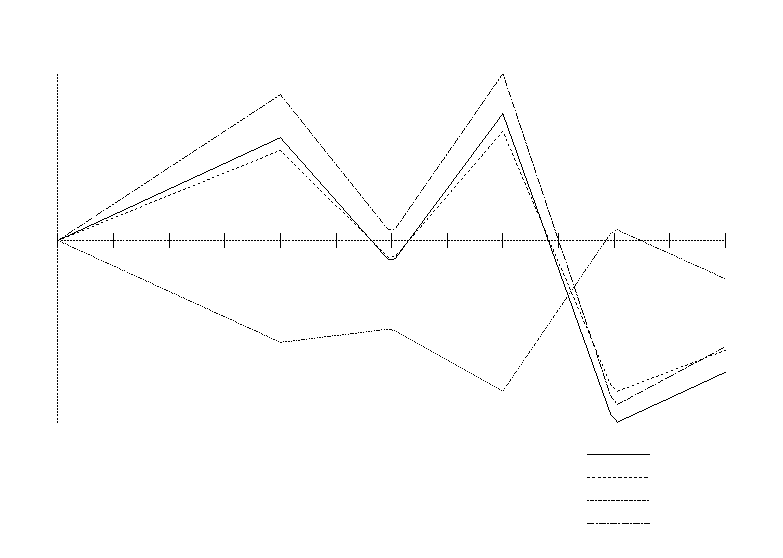
\includegraphics{fig-piecewiseIncome}}%
    \gplfronttext
  \end{picture}%
\endgroup

\caption{\label{fig:piecewiseIncome}Latent variable as a function of
  income with the estimated coefficients}
\end{figure}

\item We refer the reader to \citeasnoun{vij2016and}, who discuss the actual
  added value (or lack thereof) of using latent variables in the
  context of a choice   model. 

\end{itemize}

\clearpage

\appendix

\section{Description of the case study}

This case study deals with the estimation of a mode choice behavior
model for inhabitants in Switzerland using revealed preference data.
The survey was conducted between 2009 and 2010 for CarPostal, the public transport
branch of the Swiss Postal Service. The main purpose of this survey
is to collect data for analyzing the travel behavior of people in
low-density areas, where CarPostal typically serves. A following
study proposes new public transport alternatives according to the respondents'
willingness to pay for these potential services in order to increase
the market share of public transport.


\subsection{Data collection}

The survey covers French and German speaking areas of Switzerland. Questionnaires
were sent to people living in rural area by mail. The respondents
were asked to register all the trips performed during a specified
day. The collected information consists of origin, destination,
cost, travel time, chosen mode and activity at the destination. Moreover, we collected socio-economic information about the respondents and their households.

1124 completed surveys were collected. For each respondent,
cyclic sequences of trips (starting and ending at the same location)
are detected and their main transport mode is identified. The resulting data base includes 1906 sequences of trips linked with psychometric indicators and socio-economic attributes of the respondents. It should be noticed that each observation is a sequence of trips
that starts and ends at home. A respondent may have several sequences of trips 
in a day.

%Some socio-economic characteristics, such as gender, children and age, are also collected.
%The observations in this data set are weighted according to the statistical
%data of Switzerland considering 6 dimensions: presence of driving
%license, gender, education, number of cars in the household, age,
%and number of people in the household. These weights for individuals
%are used for having a weighted average value for the outputs of the
%model, for example cost and time elasticities in this paper, to be
%able to better represent the Swiss population.

\subsection{Variables and descriptive statistics}

The variables are described in Table \ref{tab1}. The attitudinal statements are described in Table \ref{tab:indic}. A summary of descriptive statistics for the main variables is given in Table \ref{tab8}.


Given the presence of missing data (coded as -1) an additional table summarizing the three main affected variables (TripPurpose, ReportedDuration,	age) after removing the missing cases is presented (see Table \ref{tab9}).

\clearpage


\begin{longtable}{||p{4cm}|p{9cm}||}
\caption{\label{tab1} Description of variables}\\
\hline 
\hline 
\textbf{Name} & \textbf{Description}\\
%\tabularnewline
\hline 
ID & Identifier of the respondent who described the trips in the loop.\tabularnewline
\hline 
NbTransf & The total number of transfers performed for all trips of the loop,
using public transport (ranging from 1-9).\tabularnewline
\hline 
TimePT & The duration of the loop performed in public transport (in minutes).\tabularnewline
\hline 
WalkingTimePT & The total walking time in a loop performed in public transports (in minutes).\tabularnewline
\hline 
WaitingTimePT & The total waiting time in a loop performed in public transports (in minutes).\tabularnewline
\hline 
TimeCar & The total duration of a loop made using the car (in minutes).\tabularnewline
\hline 
CostPT & Cost for public transports (full cost to perform the loop). \tabularnewline
\hline 
MarginalCostPT & The total cost of a loop performed in public transports, taking into account the ownership of a seasonal ticket by the respondent. If the respondent has a ``GA'' (full Swiss season ticket), a seasonal ticket for the line or the area, this variable takes value zero. If the respondent has a half-fare travelcard, this variable corresponds to half the cost of the trip by public transport..\tabularnewline
\hline 
CostCarCHF & The total gas cost of a loop performed with the car in CHF.\tabularnewline
\hline 
CostCar & The total gas cost of a loop performed with the car in euros.\tabularnewline
\hline 
TripPurpose & The main purpose of the loop: 1 =Work-related trips; 2 =Work- and leisure-related
trips; 3 =Leisure related trips. -1 represents missing values \tabularnewline
\hline 
TypeCommune & The commune type, based on the Swiss Federal Statistical Office 1 =Centers;
2 =Suburban communes; 3 =High-income communes; 4 =Periurban communes;
5 =Touristic communes; 6 =Industrial and tertiary communes; 7 =Rural
and commuting communes; 8 =Agricultural and mixed communes; 9 =Agricultural
communes\tabularnewline
\hline 
UrbRur & Binary variable, where: 1 =Rural; 2 =Urban.\tabularnewline
\hline 
ClassifCodeLine & Classification of the type of bus lines of the commune: 1 =Center; 2
=Centripetal; 3 =Peripheral; 4 =Feeder.\tabularnewline
\hline
frequency & Categorical variable for the frequency: 1 =Low frequency, $<$ 12 pairs
of trips per day; 2 =Low-middle frequency, 13 - 20 pairs of trips
per day; 3 =Middle-high frequency, 21-30 pairs of trips per day;
4 =High frequency, $>$ 30 pairs of trips per day.\tabularnewline
\hline 
NbTrajects & Number of trips in the loop \tabularnewline
\hline 
Region OR CoderegionCAR & Region where the commune of the respondent is situated. These regions
are defined by CarPostal as follows: 1 =Vaud; 2 =Valais; 3 =Delemont;
4 =Bern; 5 =Basel, Aargau, Olten; 6 =Zurich; 7 =Eastern Switzerland;
8 =Graubunden.\tabularnewline
\hline 
distance\_km & Total distance performed for the loop.\tabularnewline
\hline 
Choice & Choice variable: 0 = public transports (train, bus, tram, etc.); 1
= private modes (car, motorbike, etc.); 2 = soft modes (bike, walk,
etc.).\tabularnewline
\hline 
InVehicleTime & Time spent in (on-board) the transport modes only (discarding walking time and
waiting time), -1 if missing value.\tabularnewline
\hline 
ReportedDuration & Time spent for the whole loop, as reported by the respondent. -1 represents missing values\tabularnewline
\hline 
LangCode & Language of the commune where the survey was conducted: 1 =French;
2 =German.\tabularnewline
\hline 
age & Age of the respondent (in years) -1 represents missing values.\tabularnewline
\hline
DestAct & The main activity at destination: 1 is work, 2 is professional trip, 3 is studying, 4 is shopping, 5 is activity at home, 6 is eating/drinking, 7 is personal business, 8 is driving someone, 9 is cultural activity or sport, 10 is going out (with friends, restaurant, cinema, theater), 11 is other and -1 is missing value. \tabularnewline
\hline
FreqTripHouseh & Frequency of trips related to the household (drive someone, like kids, or shopping), 1 is never, 2 is several times a day, 3 is several times a week, 4 is occasionally, -1 is for missing data and -2 if respondent didn't answer to any opinion questions. \tabularnewline
ModeToSchool & Most often mode used by the respondent to go to school as a kid ($>10$), 1 is car (passenger), 2 is train, 3 is public transport, 4 is walking, 5 is biking, 6 is motorbike, 7 is other, 8 is multiple modes, -1 is for missing data and -2 if respondent didn't answer to any opinion questions. \tabularnewline
\hline 
ResidChild & Main place of residence as a kid ($<18$), 1 is city center (large town), 2 is city center (small town), 3 is suburbs, 4 is suburban town, 5 is country side (village), 6 is countryside (isolated), -1 is for missing data and -2 if respondent didn't answer to any opinion questions. \tabularnewline
\hline 
FreqCarPar & Frequency of the usage of car by the respondent's parents (or adults in charge) during childhood ($<18$), 1 is never, 2 is occasionally, 3 is regularly, 4 is exclusively, -1 is for missing data and -2 if respondent didn't answer to any opinion questions. \tabularnewline
\hline 
FreqTrainPar & Frequency of the usage of train by the respondent's parents (or adults in charge) during childhood ($<18$), 1 is never, 2 is occasionally, 3 is regularly, 4 is exclusively, -1 is for missing data and -2 if respondent didn't answer to any opinion questions. \tabularnewline 
\hline 
FreqOthPar & Frequency of the usage of tram, bus and other public transport (not train) by the respondent's parents (or adults in charge) during childhood ($<18$), 1 is never, 2 is occasionally, 3 is regularly, 4 is exclusively , -1 is for missing data and -2 if respondent didn't answer to any opinion questions. \tabularnewline
\hline
NbHousehold & Number of persons in the household. -1 for missing value. \tabularnewline
\hline 
NbChild & Number of kids ($<15$) in the household. -1 for missing value. \tabularnewline
\hline 
NbCar & Number of cars in the household.-1 for missing value. \tabularnewline
\hline 
NbMoto & Number of motorbikes in the household. -1 for missing value.\tabularnewline
\hline 
NbBicy & Number of bikes in the household. -1 for missing value.\tabularnewline
\hline 
NbBicyChild & Number of bikes for kids in the household. -1 for missing value.\tabularnewline
\hline 
NbComp & Number of computers in the household. -1 for missing value.\tabularnewline
\hline 
NbTV & Number of TVs in the household. -1 for missing value.\tabularnewline
\hline 
Internet & Internet connection, 1 is yes, 2 is no. -1 for missing value.\tabularnewline
\hline 
NewsPaperSubs & Newspaper subscription, 1 is yes, 2 is no. -1 for missing value.\tabularnewline
\hline 
NbCellPhones & Number of cell phones in the household (total). -1 for missing value.\tabularnewline
\hline 
NbSmartPhone & Number of smartphones in the household (total). -1 for missing value.\tabularnewline
\hline 
HouseType & House type, 1 is individual house (or terraced house), 2 is apartment (and other types of multi-family residential), 3 is independent room (subletting). -1 for missing value.\tabularnewline
\hline 
OwnHouse & Do you own the place where you are living? 1 is yes, 2 is no. -1 for missing value.\tabularnewline
\hline 
NbRoomsHouse & Number of rooms is your house. -1 for missing value.\tabularnewline
\hline 
YearsInHouse & Number of years spent in the current house. -1 for missing value.\tabularnewline
\hline 
Income & Net monthly income of the household in CHF. 1 is less than 2500, 2 is from 2501 to 4000, 3 is from 4001 to 6000, 4 is from 6001 to 8000, 5 is from 8001 to 10'000 and 6 is more than 10'001. -1 for missing value.\tabularnewline
\hline 
Gender & Gender of the respondent, 1 is man, 2 is woman. -1 for missing value.\tabularnewline
\hline 
BirthYear & Year of birth of the respondent. -1 for missing value.\tabularnewline
\hline 
Mothertongue & Mothertongue. 1 for German or Swiss German, 2 for french, 3 for other, -1 for missing value.\tabularnewline
\hline
FamilSitu & Familiar situation: 1 is single, 2 is in a couple without children, 3 is in a couple with children, 4 is single with your own children, 5 is in a colocation, 6 is with your parents and 7 is for other situations. -1 for missing values.\tabularnewline
\hline
OccupStat &What is you occupational status? 1 is for full-time paid
professional activity, 2 for partial-time paid professional activity,
3 for searching a job, 4 for occasional employment, 5 for no paid job,
6 for homemaker, 7 for disability leave, 8 for student and 9 for retired. -1 for missing values. \tabularnewline
\hline
SocioProfCat & To which of the following socio-professional categories do you belong? 1 is for top managers, 2 for intellectual professions, 3 for freelancers, 4 for intermediate professions, 5 for artisans and salespersons, 6 for employees, 7 for workers and 8 for others. -1 for missing values.\tabularnewline
\hline
Education &Highest education achieved. As mentioned by Wikipedia in English: "The education system in Switzerland is very diverse, because the constitution of Switzerland delegates the authority for the school system mainly to the cantons. The Swiss constitution sets the foundations, namely that primary school is obligatory for every child and is free in public schools and that the confederation can run or support universities." (source: \lstinline|http://en.wikipedia.org/wiki/Education_in_Switzerland|, accessed April 16, 2013). It is thus difficult to translate the survey that was originally in French and German. The possible answers in the survey are:
1. Unfinished compulsory education: education is compulsory in Switzerland but pupils may finish it at the legal age without succeeding the final exam.
2. Compulsory education with diploma
3. Vocational education: a three or four-year period of training both in a company and following theoretical courses. Ends with a diploma called "Certificat f\'ed\'eral de capacit\'e" (i.e., "professional baccalaureate")
4. A 3-year generalist school giving access to teaching school, nursing schools, social work school, universities of applied sciences or vocational education (sometime in less than the normal number of years). It does not give access to universities in Switzerland
5. High school: ends with the general baccalaureate exam. The general baccalaureate gives access automatically to universities.
6. Universities of applied sciences, teaching schools, nursing schools, social work schools: ends with a Bachelor and sometimes a Master, mostly focus on vocational training
7. Universities and institutes of technology: ends with an academic Bachelor and in most cases an academic Master
8. PhD thesis \tabularnewline
\hline
HalfFareST & Is equal to 1 if the respondent has a half-fare travelcard and to 2 if not.\tabularnewline
\hline
%X338 & Duration of the half-fare travelcard (1, 2, 3 years).\tabularnewline
%\hline
LineRelST & Is equal to 1 if the respondent has a line-related season ticket and 2 if not.\tabularnewline
\hline 
GenAbST & Is equal to 1 if the respondent has a GA (full Swiss season ticket) and 2 if not.\tabularnewline
\hline 
AreaRelST & Is equal to 1 if the respondent has an area-related season ticket and 2 if not.\tabularnewline
\hline
OtherST & Is equal to 1 if the respondent has a season ticket that was is not in the list and 2 if not.\tabularnewline
\hline 
CarAvail & Represents the availability of a car for the respondent: 1 is always, 2 is sometime, 3 is never. -1 for missing value.\tabularnewline
\hline 
\hline 
\end{longtable}

\clearpage

\begin{longtable}{||p{4cm}|p{9cm}||}
\caption{\label{tab:indic}Attitude questions. Coding: 1= strongly disagree, 2=disagree,
  3=neutral, 4= agree, 5= strongly agree, 6=not applicable, -1=
  missing value, -2= all answers to attitude questions missing} \\
\hline 
\hline 
\textbf{Name} & \textbf{Description}\\
%\tabularnewline
\hline 
Envir01 & Fuel price should be increased to reduce congestion and air pollution. \tabularnewline
\hline 
Envir02 & More public transportation is needed, even if taxes are set to pay the additional costs.\tabularnewline
\hline 
Envir03 & Ecology disadvantages minorities and small businesses.\tabularnewline
\hline 
Envir04 & People and employment are more important than the environment.\tabularnewline
\hline 
Envir05 & I am concerned about global warming.\tabularnewline
\hline 
Envir06 & Actions and decision making are needed to limit greenhouse gas emissions.\tabularnewline
\hline 
Mobil01 & My trip is a useful transition between home and work.\tabularnewline
\hline 
Mobil02 & The trip I must do interferes with other things I would like to do. \tabularnewline
\hline 
Mobil03 & I use the time of my trip in a productive way.\tabularnewline
\hline 
Mobil04 & Being stuck in traffic bores me.\tabularnewline
\hline 
Mobil05 & I reconsider frequently my mode choice.\tabularnewline
\hline 
Mobil06 & I use my current mean of transport mode because I have no alternative.\tabularnewline
\hline 
Mobil07 & In general, for my activities, I always have a usual mean of transport.\tabularnewline
\hline 
Mobil08 & I do not feel comfortable when I travel close to people I do not know.\tabularnewline
\hline 
Mobil09 & Taking the bus helps making the city more comfortable and welcoming.\tabularnewline
\hline 
Mobil10 & It is difficult to take the public transport when I travel with my children.\tabularnewline
\hline 
Mobil11 & It is difficult to take the public transport when I carry bags or luggage.\tabularnewline
\hline 
Mobil12 & It is very important to have a beautiful car.\tabularnewline
\hline 
Mobil13 & With my car I can go wherever and whenever.\tabularnewline
\hline 
Mobil14 & When I take the car I know I will be on time.\tabularnewline
\hline 
Mobil15 & I do not like looking for a parking place. \tabularnewline
\hline 
Mobil16 & I do not like changing the mean of transport when I am traveling.\tabularnewline
\hline 
Mobil17 & If I use public transportation I have to cancel certain activities I would have done if I had taken the car. \tabularnewline
\hline 
Mobil18 & CarPostal bus schedules are sometimes difficult to understand.\tabularnewline
\hline 
Mobil19 & I know very well which bus/train I have to take to go where I want to.\tabularnewline
\hline 
Mobil20 & I know by heart the schedules of the public transports I regularly use. \tabularnewline
\hline 
Mobil21 & I can rely on my family to drive me if needed\tabularnewline
\hline 
Mobil22 & When I am in a town I don't know I feel strongly disoriented\tabularnewline
\hline 
Mobil23 & I use the internet to check the schedules and the departure times of buses and trains.\tabularnewline
\hline 
Mobil24 & I have always used public transports all my life\tabularnewline
\hline 
Mobil25 & When I was young my parents took me to all my activities\tabularnewline
\hline 
Mobil26 & I know some drivers of the public transports that I use \tabularnewline
\hline 
Mobil27 & I think it is important to have the option to talk to the drivers of public transports.\tabularnewline
\hline 
ResidCh01 & I like living in a neighborhood where a lot of things happen. \tabularnewline
\hline 
ResidCh02 & The accessibility and mobility conditions are important for the choice of housing. \tabularnewline
\hline 
ResidCh03 & Most of my friends live in the same region I live in.\tabularnewline
\hline 
ResidCh04 & I would like to have access to more services or activities. \tabularnewline
\hline 
ResidCh05 & I would like to live in the city center of a big city.\tabularnewline
\hline 
ResidCh06 & I would like to live in a town situated in the outskirts of a city. \tabularnewline
\hline 
ResidCh07 & I would like to live in the countryside.\tabularnewline
\hline 
LifSty01 & I always choose the best products regardless of price. \tabularnewline
\hline 
LifSty02 & I always try to find the cheapest alternative. \tabularnewline
\hline 
LifSty03 & I can ask for services in my neighborhood without problems. \tabularnewline
\hline 
LifSty04 & I would like to spend more time with my family and friends. \tabularnewline
\hline 
LifSty05 & Sometimes I would like to take a day off .\tabularnewline
\hline 
LifSty06 & I can recognize the social status of other travelers by looking at their cars.\tabularnewline
\hline 
LifSty07 & The pleasure of having something beautiful consists in showing it. \tabularnewline
\hline 
LifSty08 & For me the car is only a practical way to move. \tabularnewline
\hline 
LifSty09 & I would like to spend more time working.\tabularnewline
\hline 
LifSty10 & I do not like to be in the same place for too long.\tabularnewline
\hline 
LifSty11 & I always plan my activities well in advance \tabularnewline
\hline 
LifSty12 & I like to experiment new or different situations\tabularnewline
\hline 
LifSty13 & I am not afraid of unknown people\tabularnewline
\hline 
LifSty14 & My schedule is rather regular.\tabularnewline
\hline 
\hline 
\end{longtable}



\begin{sidewaystable}[htbp]
\caption{\label{tab8} Descriptive statistics of the main variables (no data excluded) }
\vspace{0.2cm}
\begin{tabular}{||l|c|c|c|c|c|c|c||}
\hline
 & \multicolumn{1}{l|}{nbr. cases} & \multicolumn{1}{l|}{nbr. null} & \multicolumn{1}{l|}{min} & \multicolumn{1}{l|}{max} & \multicolumn{1}{l|}{median} & \multicolumn{1}{l|}{mean} & \multicolumn{1}{l|}{std.dev} \\ \hline
age & 1906 & 0 & -1 & 88 & 47 & 46.48 & 18.57 \\ \hline
Choice & 1906 & 536 & 0 & 2 & 1 & 0.78 & 0.54 \\ \hline
TypeCommune & 1906 & 0 & 1 & 9 & 6 & 5.39 & 1.99 \\ \hline
UrbRur & 1906 & 0 & 1 & 2 & 2 & 1.51 & 0.5 \\ \hline
ClassifCodeLine & 1906 & 0 & 1 & 4 & 4 & 3.17 & 0.97 \\ \hline
LangCode & 1906 & 0 & 1 & 2 & 2 & 1.74 & 0.44 \\ \hline
CoderegionCAR & 1906 & 0 & 1 & 8 & 5 & 4.58 & 2.08 \\ \hline
CostCarCHF & 1906 & 5 & 0 & 67.65 & 2.98 & 5.76 & 8.34 \\ \hline
distance\_km & 1906 & 1 & 0 & 519 & 18.75 & 40.38 & 62.6 \\ \hline
TimeCar & 1906 & 28 & 0 & 494 & 26 & 40.68 & 47.61 \\ \hline
TimePT & 1906 & 7 & 0 & 745 & 85 & 107.88 & 86.52 \\ \hline
frequency & 1906 & 0 & 1 & 4 & 3 & 2.84 & 1.09 \\ \hline
ID & 1906 & 0 & 10350017 & 96040538 & 44690042 & 45878800 & 23846908 \\ \hline
InVehicleTime & 1906 & 66 & -128 & 631 & 40.5 & 55.13 & 57.78 \\ \hline
MarginalCostPT & 1906 & 270 & 0 & 230 & 5.6 & 11.11 & 16.13 \\ \hline
NbTrajects & 1906 & 0 & 1 & 9 & 2 & 2.04 & 1.05 \\ \hline
NbTransf & 1906 & 644 & 0 & 14 & 2 & 2.01 & 2.17 \\ \hline
Region & 1906 & 0 & 1 & 8 & 5 & 4.58 & 2.08 \\ \hline
ReportedDuration & 1906 & 3 & -1 & 855 & 35 & 57.73 & 72.47 \\ \hline
TripPurpose & 1906 & 0 & -1 & 3 & 2 & 1.94 & 1.18 \\ \hline
WaitingTimePT & 1906 & 693 & 0 & 392 & 5 & 13.13 & 22.07 \\ \hline
WalkingTimePT & 1906 & 17 & 0 & 213 & 33 & 39.63 & 28 \\ \hline
\end{tabular}
\end{sidewaystable}



\begin{table}[htbp]
\caption{\label{tab9}
Descriptive statistics of the main variables affected by missing data (observations with -1 excluded)}
\vspace{0.2cm}
\begin{tabular}{|l|r|r|r|r|r|r|r|}
\hline
\multicolumn{1}{|r|}{} & \multicolumn{1}{l|}{nbr. cases} & \multicolumn{1}{l|}{nbr.null} &  \multicolumn{1}{l|}{min} & \multicolumn{1}{l|}{max} & \multicolumn{1}{l|}{median} & \multicolumn{1}{l|}{mean} & \multicolumn{1}{l|}{std.dev} \\ \hline
age & 1791 & 0  & 16 & 88 & 48 & 49.53 & 14.59 \\ \hline
ReportedDuration & 1835 & 3 & 0 & 855 & 37 & 60 & 72.92 \\ \hline
TripPurpose & 1783 & 0  & 1 & 3 & 3 & 2.14 & 0.92 \\ \hline
\end{tabular}
\end{table}

\clearpage

\section{Complete specification files}

\subsection{\lstinline$factoranalysis.r$}
\label{sec:factoranalysis}
\lstinputlisting[style=numbers]{../../../test/latent/r/factoranalysis.r}

\subsection{\lstinline$01oneLatentRegression.py$}
\label{sec:01oneLatentRegression}
\lstinputlisting[style=numbers]{../../../test/latent/01oneLatentRegression.py}

\subsection{\lstinline$02oneLatentOrdered.py$}
\label{sec:02oneLatentOrdered}
\lstinputlisting[style=numbers]{../../../test/latent/02oneLatentOrdered.py}

\subsection{\lstinline$03choiceOnly.py$}
\label{sec:03choiceOnly}
\lstinputlisting[style=numbers]{../../../test/latent/03choiceOnly.py}

\subsection{\lstinline$04latentChoiceSeq.py$}
\label{sec:04latentChoiceSeq}
\lstinputlisting[style=numbers]{../../../test/latent/04latentChoiceSeq.py}

\subsection{\lstinline$05latentChoiceFull.py$}
\label{sec:05latentChoiceFull}
\lstinputlisting[style=numbers]{../../../test/latent/05latentChoiceFull.py}

\subsection{\lstinline$06serialCorrelation.py$}
\label{sec:06serialCorrelation}
\lstinputlisting[style=numbers]{../../../test/latent/06serialCorrelation.py}


\clearpage
\bibliographystyle{dcu}
\bibliography{../dca}





\end{document}





